\documentclass[a4paper,12pt, oneside]{book}
%\usepackage{fullpage}
\usepackage[english]{babel}
\usepackage[utf8]{inputenc}
\usepackage{amssymb}
\usepackage{amsthm}
\usepackage{graphics}
\usepackage{amsfonts}
\usepackage{listings}
\usepackage{amsmath}
\usepackage{amstext}
\usepackage{colortbl}
\usepackage{engrec}
\usepackage{appendix}
\usepackage{multicol}
\usepackage{rotating}
\usepackage{subcaption}
\usepackage{verbatim}
\usepackage{stackengine}
\usepackage[safe,extra]{tipa}
% \usepackage{showkeys}
\usepackage{multirow}
\usepackage{hyperref}
\usepackage{microtype}
% \usepackage{fontspec}
\usepackage{enumerate}
\usepackage{braket}
\usepackage{relsize}
\usepackage{marginnote}
\usepackage{pgfplots}
\usepackage{cancel}
\usepackage{polynom}
\usepackage{booktabs}
\usepackage{enumitem}
\usepackage{framed}
\usepackage{pdfpages}
\usepackage{pgfplots}
\usepackage[chapter]{algorithm}
%\usepackage[ruled,vlined,linesnumbered]{algorithm2e}
%\usepackage[ruled,vlined]{algorithm2e}
\makeatletter
\renewcommand{\ALG@name}{Algoritmo}
%\renewcommand{\listalgorithmname}{Lista degli algoritmi}
\makeatother
%\usepackage[backend=biber, backref=true, sorting=none]{biblatex}
\usepackage{fvextra}
\usepackage{csquotes}
% \usepackage{natbib}
% \usepackage{algpseudocode}
%\usepackage[cache=false]{minted}
\usepackage{mathtools}
\usepackage[noend]{algpseudocode}
\usepackage{svg}
\usepackage{graphicx}
\usepackage{hyperref}
\usepackage{setspace}
\usepackage{geometry}
\usepackage{blindtext}
\usepackage{titleps}
%\usepackage{graphicx}
\usepackage{wrapfig}
\setlength{\headheight}{15pt}
%\usepackage[ backend=biber,%style=alphabetic, sorting=ynt ]{biblatex}\addbibresource{reference.bib}
\usepackage{enumitem}
\renewcommand{\labelenumii}{\arabic{enumi}.\arabic{enumii}}
\renewcommand{\labelenumiii}{\arabic{enumi}.\arabic{enumii}.\arabic{enumiii}}
\renewcommand{\labelenumiv}{\arabic{enumi}.\arabic{enumii}.\arabic{enumiii}.\arabic{enumiv}}

% \makeatletter
% \long\def\@makecaption#1#2{%
%   \vskip\abovecaptionskip
%     \bfseries #1: #2\par
%   \vskip\belowcaptionskip}%
% \makeatother
% \lstset{ % General setup for the package
%     language=Perl,
%     basicstyle=\small\sffamily,
%     frame=lines,
%     tabsize=4,
%     columns=fixed,
%     showstringspaces=false,
%     showtabs=false,
%     keepspaces,
%     commentstyle=\color{red},
%     keywordstyle=\color{blue}
% }
% \usepackage{tikz}\usetikzlibrary{er}\tikzset{multi  attribute /.style={attribute
%     ,double  distance =1.5pt}}\tikzset{derived  attribute /.style={attribute
%     ,dashed}}\tikzset{total /.style={double  distance =1.5pt}}\tikzset{every
%   entity /.style={draw=orange , fill=orange!20}}\tikzset{every  attribute
%   /.style={draw=MediumPurple1, fill=MediumPurple1!20}}\tikzset{every
%   relationship /.style={draw=Chartreuse2,
%     fill=Chartreuse2!20}}\newcommand{\key}[1]{\underline{#1}}
% \usetikzlibrary{arrows.meta}
% \usetikzlibrary{decorations.markings}
% \usetikzlibrary{arrows,shapes,backgrounds,petri} 
% \usetikzlibrary{automata,positioning}
% \usetikzlibrary{matrix}

%\usepackage[textsize=scriptsize, textwidth = 25mm]{todonotes}
\usepackage[disable, textsize=scriptsize, textwidth = 25mm]{todonotes}


% \renewcommand{\chaptermark}[1]{\markboth{#1}{}}
\usepackage{fancyhdr}
\pagestyle{fancy}

\fancyhead[LO,RE]{\slshape \leftmark}
% \fancyhead[CO,CE]{\slshape\rightmark}
\fancyhead[LE,RO]{\slshape\rightmark}
\fancyfoot[C]{\thepage}
% \fancyhf{}
% \fancyhead[LO,RE]{\slshape \leftmark}
% % \fancyhead[CO,CE]{\slshape\rightmark}
% \fancyhead[LE,RO]{\slshape\thepage}
% \renewcommand{\footrulewidth}{0pt}
% \fancyfoot[C]{\thepage}
% \title{Relazione}
% \fancypagestyle{plain}{% \fancyhf{} % clear all header and footer fields
% \fancyhead[RO,RE]{\thepage}%RO=right odd, RE=right even
% \renewcommand{\headrulewidth}{0pt}
% \renewcommand{\footrulewidth}{0.3pt}}

% \AtBeginDocument{%
%   \renewcommand{\thelisting}{\Alph{chapter}.\arabic{listing}}
%   % \renewcommand\thetable{\Alph{section}.\arabic{table}}
%   % \renewcommand\thefigure{\Alph{section}.\arabic{figure}}
% }
% %Automatically change the driver counter for reset:
% \makeatletter
% \g@addto@macro\appendix{%
%   \counterwithin*{listing}{section}%
% }
% \makeatother
% c C plus plus
\def\Cplusplus{C\raisebox{0.5ex}{\tiny\textbf{++}}}
\definecolor{nordred}{RGB}{191, 97, 106}
\definecolor{nordcyan}{RGB}{94,129,172}
\definecolor{nordgreen}{RGB}{135, 157, 116}
\definecolor{nordpurple}{RGB}{180,142,173}

\pgfplotsset{compat=1.13}
\setlist[itemize]{leftmargin=.5in}
\setlist[enumerate]{leftmargin=.5in}
\begin{document}

% \maketitle
\newgeometry{margin=1in} 
\begin{titlepage}
  

  \noindent
  \begin{minipage}[t]{0.19\textwidth}
    \vspace{-4mm}{
\includegraphics[scale=1.15]{img/logo_unimib.pdf}}
  \end{minipage}
  \begin{minipage}[t]{0.81\textwidth}
    {
      \setstretch{1.42}
      {\textsc{Università degli Studi di Milano - Bicocca}} \\
      \textbf{Scuola di Scienze} \\
      \textbf{Dipartimento di Informatica, Sistemistica e Comunicazione} \\
      \textbf{Corso di Laurea Magistrale in Informatica} \\
      \par
    }
  \end{minipage}
  
  \vspace{40mm}
  
  \begin{center}
    {\LARGE{
        \setstretch{1.2}
        \textbf{Respiratory Rate Estimation using a\vspace{5mm}}}}
    %\vspace{5mm}
    {\LARGE{
        \setstretch{1.2}
        \textbf{ Pressure Sensor Mattress}}}
 %   \vspace{1mm}
  %  {\LARGE{
   %     \setstretch{1.2}
    %    \textbf{compressione run-length}}}
    
  \end{center}
  
  \vspace{43mm}

  \noindent
  {\large \textbf{Relatore:} \textit{Prof.~Domenico Sorrenti}} \\

  \noindent
  {\large \textbf{Correlatore:} \textit{Prof.~Cristiano Alessandro}}
  
  \vspace{15mm}

  \begin{flushright}
    \textbf{\large Tesi di Laurea Magistrale di:} \\
    \large{\textit{Artemisia Sarteschi}}\\
    \large{\textit{Matricola 829677}}
  \end{flushright}
  
  \vspace{25mm}
  \begin{center}
    {\large{\bf Anno Accademico 2021-2022}}
  \end{center}

  \restoregeometry
  
\end{titlepage}
\restoregeometry
\definecolor{shadecolor}{gray}{0.80}
\setlist{leftmargin = 2cm}
\newtheorem{teorema}{Teorema}
\newtheorem{definizione}{Definizione}
\newtheorem{esempio}{Esempio}
\newtheorem{corollario}{Corollario}
\newtheorem{lemma}{Lemma}
\newtheorem{osservazione}{Osservazione}
\newtheorem{nota}{Nota}
\newtheorem{esercizio}{Esercizio}

\algdef{SE}[DOWHILE]{Do}{doWhile}{\algorithmicdo}[1]{\algorithmicwhile\ #1}
\renewcommand{\chaptermark}[1]{%
  \markboth{\chaptername
    \ \thechapter.\ #1}{}}
\renewcommand{\sectionmark}[1]{\markright{\thesection.\ #1}}
\newcommand{\floor}[1]{\lfloor #1 \rfloor}

\newcommand{\MYhref}[3][blue]{\href{#2}{\color{#1}{#3}}}%
\newcommand{\hiddenchapter}[1]{
  \stepcounter{chapter*}
  \chapter*{\arabic{chapter}\hspace{1em}{#1}}
}
\newcommand\xrowht[2][0]{\addstackgap[.5\dimexpr#2\relax]{\vphantom{#1}}}
% \pagenumbering{roman}
\begin{titlepage}
  \begin{flushright}
    \textit{Quando la vita si fa dura sai che devi fare Marlin? \\ Zitto e nuota, nuota e nuota, zitto e nuota e nuota e nuota? \\ E noi che si fa? \\ Nuotiam, nuotiam…. \\   Dory }
  \end{flushright}
\end{titlepage}
\newpage
\newpage
% \thispagestyle{plain}
% \begin{flushleft}
%   \huge{\textbf{Abstract}}
% \end{flushleft}
% \vspace{10mm}
% \input{include/abstract}
{
  \pagestyle{plain}
  \tableofcontents
  \cleardoublepage
}

% CAPITOLI
%\chapter*{Abstract}
Sleep is one of the most important physiological functions. Sleep quality can affect physical and mental wellness; for this reason,
 it is crucial to monitor vital signs without interfering with natural sleep. 
 The state-of-the-art to monitor physiological data during sleep is cardio-respiratory polysomnography, which involves a cannula, chest belts and electrodes for ECG.

 During sleep, a person cycles between two phases Non-Rapid Eye Movement (NREM) and Rapid Eye Movement (REM); this second phase is further divided into three other stages (N1-N3). Different muscle tones, brain wave patterns, eye movements, and heart and breathing rate alterations characterise every phase and stage.
\textbf{[explenation of sleep stages]}.
Focusing on one of the vital signs that characterise the different sleep stages is the respiratory rate which slowly becomes more stable going from the awake to the REM phase. Respiration is also central in one of the most common sleep disorders, sleep apnea, in this case, the individuals experience a collapse of the airway in deeper sleep states, causing them to experience reduced time in stage N3 and REM sleep. 
The ability to monitor it allows for a faster and closer intervention in severe cases. 

As said before, the state-of-art is a cumbersome device that 
requires cables attached to the users' bodies and often interferes with 
natural sleep. For this reason, we decided to use an unobtrusive sensor 
placed over the typical mattress to allow us to study the possibility of
 monitoring the patient's health. The sensor involved in this project is a 
 pressure-sensor textile from SensingTex [x], with a sensor area of 192 x 94 
 cm filled with 1056 sensors (sensor area density of 4 sensors for 10cm$^2$).

 The high number of sensors leads to the necessity of an algorithm to discriminate the ones from whom it is possible to extract valuable information about the respiratory rate of the person that is on the mattress.
 Many of these channels are with null or stationary information; others present just interference from the mattress itself. From just a few sensors, it is possible to retrieve a respiratory pattern and extract the respiratory rate per minute (rpm). To obtain them from all the possibilities, we have defined our confidence metric to assign each sensor a percentage of confidence that it will be a suitable sensor.
 \textbf{[parlare del somnomat]}.

 Since no data and polygraphs were available from the same person
 on the SensingTex was necessary to collect new data, this gives 
 us the possibility also to understand if this kind of Instrument
  could work with a lab project called Somnomat. A special 
  rocking bed \textbf{[parlare del somnomat e di come potrebbe essere integrato]}. The protocol involved 6 participants (three female /three male) between 20-30 years of age. It was divided into two phases: one with the sensor mattress over a standard bed and the second on the rocking bed while this was moving. Each participant had a fixed set of positions that had to be while lying on the mattress. We also decide to insert variability into the data since, during sleep, respiratory rate increases in different stages. In order to do that, we ask a participant to perform a set of five jumps before lying down in the first phase of the protocol; for the second part, we ask them to turn around on the bed and stay on it 
  while it is moving without performing any activity.


  the data collection also involved Cardiorespiratory polysomnography. In our case, we use the nox a1 and noxturnal app. 
  \textbf{chennal selected and canulas}

  x---x

  the data coming from the data collection was cleaned in this methods, than was used this approach to smoot or filtering the singal.
  than was use this to asset the number of breath



  %- introduci il problema
%- due righe di stato dell'arte
%- quali erano gli obiettivi
%- cosa hai fatto

\chapter{Introduction}


This work aims to investigate the possibility of estimating a patient's respiratory rate using a sensor pressure mattress and whether its usage with a rocking bed could hamper reaching this objective. 
Initially, the possibility of extracting the breath and heart rate from pressure sensors has been investigated using a dataset already available from previous studies. The work, therefore, will focus on respiratory rate. Since the necessary data are not available, data collection has been conducted using an innovative textile pressure sensor mattress and cardiorespiratory polysomnography as ground truth: the primary objective has been to collect data in order to understand the feasibility of determining breath rate from the mattress in case of stationary bed; the second goal has been to understand if the movement of the rocking bed could influence the measurement of the breathing rate. 
Then a pipeline has been created to analyse the extracted data: from each mattress sensor, the signals are processed to exclude the ones without meaningful information, such as those where the person is not present. Metrics have been designed to assess the confidence that a respiratory pattern could be extracted from a sensor. The selected signals are filtered to eliminate noise using multiresolution analysis of the maximal overlap discrete wavelet transform and Savitz-Golay filter to obtain a clean wave from which the number of breaths a person has in a minute could be counted. As a result, the respiration rate per minute of the person has been obtained and compared with the cardiopulmonary polysomnography to assess the error. The influence of the rocking bed on the mattress has been obtained by comparing the mattress's performance with the stationary bed. As a result of the pipeline, a heatmap, has been made available to visualise where the best sensors are positioned with respect to the body and mattress. \newline

Sleep is one of the most important physiological functions. Sleep quality can affect physical and mental wellness; for this reason, it is crucial to monitor vital signs and sleep stages without interfering with natural sleep. 
The state-of-the-art in sleep monitoring technology for physiological data is polysomnography \cite{Penzel2016ModulationsPolysomnography}, which involves recording sleep stages, respiratory and heart rate, and other parameters. However, this procedure is time-consuming, complicated, expensive, invasive for the patient and often unavailable in hospitals. Even in its simplified version, cardiorespiratory polysomnography \cite{CallejaComparisonApnoea}, where only nose cannulas, chest belts and electrocardiogram (ECG) electrodes are involved and neurophysiological variables are not tracked, the patient is subjected to physical discomfort throughout the night.

Breathing monitoring is also crucial because the population presents a higher percentage of sleep-related breathing disorders that can be studied and monitored with this instrument, like sleep apnoea/hypopnoea syndrome (SAS)\cite{SasPatients},  where the individuals experience a collapse of the airway in deeper sleep states: the ability to monitor it allows for a faster and closer intervention in severe cases. 

Also, in the study of sleep stages \cite{Gasmi2020SleepVariables}, it is known that different muscle tones, brain wave patterns, eye movements and heart and breathing rate alterations characterise every phase and stage.
In particular, the respiratory rate slowly becomes more stable in the Non-Rapid Eye Movement (NREM) phase and increases during the Rapid Eye Movement (REM) phase, giving the possibility to understand at which stage a person is just by focusing on the respiratory signal\cite{Pal2022BreathingWakefulness}.

%So if focused on one of the vital signs that characterise the different sleep stages, like  this characterisation of the different stages gives the possibility 

Nowadays, it is possible to achieve this goal using different unobtrusive methods, such as radar technology \cite{RadarSensor}. The limitation of this approach lies in the fact that the presence of another person in the room, in a hospital condition like a nurse or doctor, or even from fans or oxygen concentrators, could be a source of noise for the radar that could lead to an incorrect prediction; it can also be disturbed by the movement of the patient itself \cite{LauteslagerValidation}. Another possibility is to use video cameras with infrared filters \cite{CamerasBasedVitalSigns}; even if this approach seems promising, it leads to personal privacy concerns. 
Currently, it is possible to buy smartwatches, like Garmin\cite{garminUrl}, that can estimate multiple vital signs with good precision\cite{GarminArticol}, but they need to be worn all night, which could lead to discomfort for some people.
Moreover, these devices do not allow raw data extraction, and tracking is lost if the batteries run out. It is also possible to find under-mattress ballistocardiography-based sensors\cite{Tenhunen2013EmfitBreathing}, like Emfit \cite{emfitUrl}, that in case of multiple people inside the bed need to be placed in half of it and the wrong position can lead to inaccurate data.

In this thesis, it has been decided to use unobtrusive methods not to cause discomfort to the user, which could also give us the possibility to track vital signs. 

However, the decision of which type of method to use has been influenced by the availability, in the lab where this thesis has been carried out, of a rocking bed part of the \textit{Somnomat}\cite{DevelopingSleep} project. This rocking bed aims to interact with the person and study how to improve sleep quality via vestibular stimulation. Also, in this case, the possibility of tracking vital signs could be significant, so the possibility of integrating unobtrusive methods with the Somnomat is part of this thesis.
Given all those considerations, the choice fell to pressure sensor mattresses (hereafter referred to as ``pressure mattresses'').
They can be installed over the standard mattress and are now available as textile-sensor, which means that they can be very thin and lead to negligible discomfort, but at the same time, can be used to track the respiratory rate and, depending on the sensor area density and sampling frequency of the sensors, even heart rate. 

In this project, at first, it has been decided to use pressure-sensor textile mattresses from \textit{Sensomative} \cite{sensomativeUrl} that have 14 x 28 sensor elements for a total sensor area of 40cm x 80cm that can cover a width of a regular bed with a sampling rate of 50Hz. Due to the small area of this pressure mattress, it needs to be placed in a specific position and in case the patient moves, it is not possible to have any data. Previous studies have brought out the possibility of estimating breathing patterns; since the data from this mattress and the ground truth data from polysomnography are available, this possibility is explored.

After evaluating a possible valid approach to this data, it has been decided to use it on a second mattress, from \textit{SensingTex} \cite{SensingConnectivity} that is already installed in a hospital ward of the \textit{University of Bern} for the study research on movement disorders during sleep in patients with Parkinson’s disease. The ability to estimate breath and heart rate could be helpful for that study.
This mattress has a sampling frequency of 10Hz and 40 x 22 sensor elements for a total area of 192cm x 94cm that can cover a standard bed's area.

Raw data extracted from the mattress can be visualized to determine the person's position and movement, and it is shown as a heatmap since pressure sensors record the different pressures exerted by the presence/absence of a body or by its parts on it. 

%insert part image to make understand 
So it has been possible to create a heatmap to show the variation in colour of the intensity of the pressure, which can produce the shape of a person on the mattress.
Looking closer into signals of single channels is possible to see a pattern that resembles a breathing rhythm, similar to the data that can be retrieved from the nasal pressure exerted on the cannula of cardiorespiratory polysomnography.
This pattern was the key factor in deciding to use this pressure mattress. 


Since there is no data on the rocking bed recorded before this project, it has been necessary to conduct a data collection with two main objectives: the primary has been to collect data to understand the feasibility of extracting breath rate from the mat; the second goal has been to understand if the movement of the rocking bed could influence the signal.
Six people participated in the data collection, half male and half female, between 20 and 30 years old.
Each participant wears a cardiorespiratory wireless and portable polysomnography device (Nox A1 PSG by Nox Medical\cite{WirelessSystem}) that monitors nasal pressure, pulse, and heart rate with ECG and respiratory inductance plethysmography (RIP), which is a method of evaluating pulmonary ventilation by measuring the movement of the chest and abdominal wall. 

The protocol has been divided into two phases:
\begin{itemize}
\item The setting for the first phase involved placing the pressure mat over a standard bed. During the night and through the different sleep stages, the breath rate increases or decreases, so it has been decided to insert a similar variability in the data. The participant had to perform a set of five jumps and then lie down in a specific position for four minutes. After this period, they had to stand up, repeat the five jumps and lie down again. The positions follow a pattern of supine, left side, prone, right side and with a total of twenty jumps.


\item For the second phase, since the data needs to be collected while the Somnomat is moving, the period for the movement of the bed has been fixed at 4 seconds (15 periods in a minute) with an acceleration of 0.25 $m/s^2$. Also, in this phase, the participants were asked to turn around following the specific pattern: supine, left side, prone, right side and remain in that position for 4 minutes.
\end{itemize}
This resulted in a recording of 32 minutes for each participant divided into 4 minutes in each of the four positions with a standard bed and with Somnomat.


The SensingTex has a total of 1056 sensors, but they are never all significant at the same time. A person's body can not cover the entire mattress and activate all the sensors (hereafter referred to as ``Channels") simultaneously. Consequently, this leads to the necessity of an algorithm to discriminate the ones from where it has been possible to extract valuable information.
Many of these channels are stationary on a value; others present just interference from the mattress. It has been possible to retrieve a respiratory pattern from just a few sensors and then extract the respiratory rate per minute (rpm). Therefore becomes necessary to design a metric that underlines these channels. 
This metric must be interpreted as confidence expressed in percentual of the goodness of the signal; at the same time, it is necessary to have a workflow that can estimate a person’s respiratory rate from mattress data. This led to the creation of a pipeline that estimates the rpm based on the previous minute. The objective is to create a real-time pipeline in which the streaming of the sensors is simulated with a 60-second long moving window that slides with an interval of 10 seconds on the data collected in the project.


The first step of the pipeline excludes those signals for the entire window length that are either stationary or present only interference from the mattress.
 That interference appears as spikes but sometimes is present just in a percentage of the signal; the same could happen for stationarities that can be focused in just a subpart of the windows. In this case, the signal has been not excluded and has been assigned with confidence equal to the percentage of the signal that could have meaningful information.
 Another possibility is a noisy signal, excluded or weighted with a percentage of confidence with the same approach as the previous two.
 
 After these preliminary analyses, the number of signals decreases drastically.
 It has been assumed to count as one breath the moment between inhaling and exhaling, which can also be considered a peak in the signal wave.
 At this point, most of the signals are still noisy. To be better analysed, it has been decided to filter them using two different approaches: Multiresolution analysis of the maximal overlap discrete wavelet transform and Savitz-Golay filter.


 The reconstructed signals are given as input to a peak finder algorithm to select both peaks and valleys of the signal. 
 The channels with peaks greater than 30 rpm are excluded because the normal rpm during sleep is between 8-25rpm \cite{Chourpiliadis2022PhysiologyRate}, but since a rate over 25rpm is predictive of cardiopulmonary arrest \cite{yuan2013respiratory}, it has been decided to keep only signals under 30rpm.
 The remaining signals are further analyzed in their structure to understand whether they represent a breath pattern.
 
 In the end, to calculate the rpm, the channels with the highest confidence percentage are taken into account, and the rpm has been computed as the average of the number of peaks of the signals. A heatmap has also been visualized in the different moments to understand where the best channels are in respect of the body depending on the position. 









 % \cite{Bakker2021EstimatingSeverity}. 
%Respiration is also central in 
% one of the most common sleep disorders, sleep apnea, in this case, causes them to experience reduced time in stage N3 and REM sleep. si può every da 



\subsubsection*{indice in forma discorsiva \\ lo compilo come ultime cosa}

\subsection*{Acknowledgement}
The project is carried out in collaboration with \textit{Sensory-Motor System Lab} of Prof.~Robert Riener at \textit{Eidgenössische Technische Hochschule 
(ETH) Zürich} and supervised by Dr.~Alexander Breuss, Dr.~Oriella Gnarra and Dr.~Manuel Fujis\cite{ManuelZurich}.




\newpage
\begin{comment}
\begin{enumerate}
    \item  \textbf{Introduzione} \\  strutturato in 3 parti: 0.5 a 1 pagina di super-short-intro,descrive cosa è stato fatto dando anche il contesto (con citazioni) e riassunto di cosa ci sarà nei capitoli
    \item \textbf{State of Art} \\ contiene al suo interno tutta la parte di stato dell'arte dei seguenti argomenti e tutte le informaizoni necessarie per comprendere la tesi.
    \begin{enumerate}
        \item \textbf{Sleep Stages} \\ Il progetto nasce nel contesto di avere la necessita di poter monitorare la respirazione dei pazienti durante la notte, dalla letteratura si evince come la variazione nella respirazione possa essere usato per tracciarli.
        \item \textbf{Respiratory Rate} \\ Parlando di repirazione durante la tesi è necessario introdurre come funzioni la respirazione e come si definisca un respiro.
        \item \textbf{Caridiorespiratory Polysomnography} \\ Come si effettuano ad oggi i montoraggi delle respirazione in ospedale, evidenzaindone i limiti.
        \item \textbf{Unobstrusive approaches} \\ citazione di altri sistemi usati ora, non ustrusivi e i motivi per cui non si vogliano usare nel nostro caso
        \item \textbf{Pressure Sensor Mattress} \\ stato ell'arte di cosa si possa fare con i materassi a pressione e similari
    \end{enumerate}
    \item \textbf{Methods} 
    \begin{enumerate}
        \item \textbf{Instrument} \\ strumenti coinvolti nella tesi
            \begin{enumerate}
                \item \textbf{Sensomative} \\ materasso piccolo bello 50hz
                \item \textbf{SensingTex} \\ materasso grande brutto 10hz
                \item  \textbf{Polysomnography NOXA1} \\ utilizzata per tracciare la respirazione del soggeto
                \item \textbf{Somnomat} \\ letto che si muove, si vuole capire se sia utilizzabile insieme al materasso
            \end{enumerate} 
        \item  \textbf{Preliminary Study of different approaches} \\ approccio preliminare effettuato sui dati del materasso piccolo bello per estrarre respirazione e battito caridaco.
        \item  \textbf{Data Collection} \\ descrizione della necessità di avere dati per poter studiare la possibilitò di estrarre il ritmo respiratorio
            \begin{enumerate}
                \item \textbf{Normal Bed} \\ letto normale, le persone fanno 4 salti e poi si sdraiano in 4 posizioni diverse (totale 16 salti). serve per avere variabilità nei dati
                \item  \textbf{rocking bed, somnomat } \\ letto che si muove, persona sdraiata sopra che si gira in 4 posizioni, serve per vedere possibili alterazioni nei dati dovute dal movimento del letto
            \end{enumerate}  
    \end{enumerate}  
    \item  \textbf{Data Analysis} \\ Descrizione della pipeline, dai dati del materasso, preprocessamento, filtri vari, al numero di respiri al minuto per quel specifico minuto.
    \begin{enumerate}
        \item \textbf{Weighted and binary} \\ la pipeline viene creata sia dando un peso ai vari controlli effettuati sul segnale, sia rendendoli binari (o passa o non passa)
        \item  \textbf{Pipeline} \\ Descrizione effettiva della pipeline
        \begin{enumerate}
            \item \textbf{Excluding criteria} \\ criteri di esclusione dei canali, non si effettuano ulteriori analisi.
            \item  \textbf{SNR ratio} \\ deve rimanere in un intervallo, però avevo fatto casino inserendolo quindi non so se voglio citarlo
            \item  \textbf{Wavelet} 
            \begin{enumerate}
                \item teoria di come funziona
                \item applicazione nel progetto
            \end{enumerate} 
            \item \textbf{Savitz-Golay filter}
            \begin{enumerate}
                \item teoria di come funziona
                \item applicazione nel progetto
            \end{enumerate} 
            \item \textbf{Subsequent analyses of the filtered signa} \\ analisi sul segnale filtrato, controllo del numero di respiri, controllo della distanza tra picchi e valli che viene intesa sia come durata (distanza sull'asse del tempo in un intervallo +-20\%) oppure distanza euclidea picco valle (sempre +- 20\%).
        \end{enumerate} 
        \item \textbf{Result of the Pipeline (visual)} \\ risultati visuali ottenuti dalla pipeline. quidni la possibilità di visualizzare dove son i canali migliori e farci delle considerazioni.
    \end{enumerate} 
    \item \textbf{Result}
    \begin{enumerate}
        \item \textbf{Evaluation Metrics} \\spiegazione delle metriche utilizzate e la motivazione
        \begin{enumerate}
            \item Mean absolute error (MAE)
            \item Mean absolute percentage error (MAPE)
            \item Root Mean Square Error (RMSE)
        \end{enumerate} 
        \item \textbf{Result for Wavelet}
        \begin{enumerate}
            \item Bland-Altman plot 77durante la discussione su mi hanno detto che è meglio utilizzare questi per raprpesentare i risultati. ma avendo pochi dati non saprei
        \end{enumerate} 
        \item \textbf{Result for sg filter}
        \begin{enumerate}
            \item Bland-Altman plot
        \end{enumerate} 
        \item \textbf{Comparison between the two approaches (wavelet and SG filter)} \\ piccolo commento su una che va meglio dell'altro, sg filter >> wavelet
        \item  \textbf{Discussion performance on normal vs rocking bed)} \\ spiegre che funziona comnque a prescindere
    \end{enumerate} 
    \item \textbf{Conclusion and future discussin} \\ gli ampliamenti futuri ed un sunto sul fatto che si possa usare
\end{enumerate}
\end{comment}

\chapter{State of Art}
\section{Sleep Stages}
For this reason, it is nowadays 
acceptable to use cardiorespiratory polysomnography that does not track neurophysiological variables. This type of polysomnography
involves a cannula, chest belts and electrodes for an electrocardiogram (ECG) but does not involve an electroencephalogram (EEG).
Another reason why this kind of instrument is widely used is that inside the population, we have a higher percentage of 
sleep-related breathing disorders that can be studied and monitored with this instrument, like sleep apnoea/hypopnoea syndrome (SAS), 
where the individuals experience a collapse 
of the airway in deeper sleep states. The ability to monitor it allows for a faster and closer intervention in severe cases. 
The sleep cycle of a person is divided into two phases Non-Rapid Eye Movement (NREM) and Rapid Eye Movement (REM);
this second phase is further divided into three other stages (N1-N3). Different muscle tones, brain wave patterns, 
eye movements, and heart and breathing rate alterations characterise every phase and stage.
\section{Respiratory Rate}
The state-of-the-art to monitor physiological data during sleep is polysomnography \cite{Penzel2016ModulationsPolysomnography}
, which involves recording sleep stages, respiratory rate, heart and other parameters. However, this procedure is time-consuming, 
complicated, expensive, invasive for the patient and only sometimes available in hospitals. 
%\textbf{[explenation of sleep stages]}.
Focusing on one of the vital signs that characterise the different sleep stages is the respiratory rate 
which slowly becomes more stable going from the awake to the REM phase; this characterisation of the different stages gives the possibility to 
understand in which stage a person is based just on the respiratory signal.
\section{Polysomnography}
\section{Pressure Sensor Mattress}
As said before, the state-of-art is a cumbersome device that requires cables attached to the users' bodies and often interferes with natural sleep. To avoid it, in literature is possible to find new instruments like video cameras which lead to privacy concerns, radar technology that could have problems in case there are more than one person inside the room or smartwatches that are also able to track respiratory rate but involve to have something on the arm that still can lead to discomfort.


%%
    Sleep is one of the most important physiological functions. Sleep quality can affect physical 
    and mental wellness; for this reason,
    it is crucial to monitor vital signs without interfering with natural sleep. 
    The state-of-the-art to monitor physiological data during sleep is polysomnography \cite{Penzel2016ModulationsPolysomnography}
    , which involves recording sleep stages, respiratory rate, heart and other parameters. However, this procedure is time-consuming, 
    complicated, expensive, invasive for the patient and only sometimes available in hospitals. For this reason, it is nowadays 
    acceptable to use cardiorespiratory polysomnography that does not track neurophysiological variables. 
    This type of polysomnography
    involves a cannula, chest belts and electrodes for an electrocardiogram (ECG) but does not involve an electroencephalogram (EEG).
   
    Another reason why this kind of instrument is widely used is that inside the population, we have a higher percentage of 
    sleep-related breathing disorders that can be studied and monitored with this instrument, like sleep apnoea/hypopnoea syndrome (SAS), 
    where the individuals experience a collapse 
    of the airway in deeper sleep states. The ability to monitor it allows for a faster and closer intervention in severe cases. 
    The sleep cycle of a person is divided into two phases Non-Rapid Eye Movement (NREM) and Rapid Eye Movement (REM);
    this second phase is further divided into three other stages (N1-N3). Different muscle tones, brain wave patterns, 
    eye movements, and heart and breathing rate alterations characterise every phase and stage.
    %\textbf{[explenation of sleep stages]}.
    Focusing on one of the vital signs that characterise the different sleep stages is the respiratory rate 
    which slowly becomes more stable going from the awake to the REM phase; this characterisation of the different stages gives the possibility to 
    understand in which stage a person is based just on the respiratory signal.
     % \cite{Bakker2021EstimatingSeverity}. 
    %Respiration is also central in 
    % one of the most common sleep disorders, sleep apnea, in this case, causes them to experience reduced time in stage N3 and REM sleep. si può every da 
    As said before, the state-of-art is a cumbersome device that requires cables attached to the users' bodies and often interferes with natural sleep. To avoid it, in literature is possible to find new instruments like video cameras which lead to privacy concerns, radar technology that could have problems in case there are more than one person inside the room or smartwatches that are also able to track respiratory rate but involve to have something on the arm that still can lead to discomfort.
    
    
    \subsection*{Instruments}
    For this reason, this thesis aims to study the possibility to use an unobtrusive sensor placed over the usual mattress to retrieve 
    respiratory rate without discomfort for the person lying down on it. 
    
    
    The sensors in this project appear like a thin mattress similar in size to a common one that can be easily installed with adjustable straps.
    In particular, the sensors are pressure-sensor textiles from \textit{SensingTex®}; in our case, was used the Pressure Mat Dev Kit,
     that has a sensor area of 192 x 94 cm filled with 1056 sensors (hereafter also referred to as "Channels") sampled at 250hz
     with a total sensor area density of 4 sensors for 10cm$^2$.
     The raw data extracted from the mattress can be viewed together to visually see the position of the person since the sensors are pressure sensors
    the different pressures exerted by the presence/absence of a body on it or by its parts are given as a number inside an interval. 
    So it is possible to create a heat map (or heatmap) to show the variation in colour of the intensity of the pressure, which can create the shape of
    a person on the mattress.
    
    Looking closer into signals of singles channels is possible to see a pattern that resembles a breathing rhythm,  similar to the data that can
     be retrieved from the nasal pressure exerted on the cannula of cardiorespiratory polysomnography.
    This pattern was the key factor in deciding to use this sensor mattress (hereafter also referred to as "Sensor Mat" or "Mat"). 
    In the laboratory where this project was carried on, was available a rocking bed (Somnomat) involved in a study of an intervention for 
    sleep apnea, it was decided to address another question or if it is possible to retrieve the respiratory rate while the rocking bed is moving.
    The possibility of integrating SensingTex® with Somnomat could be significant to have a closer and faster intervention on sleep apnea.
    
    \subsection*{Data Collection}
    The primary objective of this study is to collect data to understand the feasibility of extracting breath rate from the mat; the second goal is to understand if the movement of the rocking bed could influence the signal.
    The participant involved was 6, half male and half female, between 20-30 years old, who were asked to lie on a standard mattress covered with the sensor mattresses in a specific position. 
    After the 4 minutes, they were asked to turn around in another position following a specific pattern: supine, left side, prone, right side.
    Each participant wore a cardiorespiratory wireless and portable polysomnography device (Nox A1 PSG of Nox Medical) that was
    monitoring respiratory inductance plethysmography (RIP) which is a method of evaluating pulmonary ventilation by measuring the movement of the chest and abdominal wall, nasal pressure, pulse and heart rate with ECG. 
    The study was divided into two phases:
    
    The setting for the first phase involves the pressure mat over a standard bed. During the night and through the different sleep stages, the breath rate increase or decreases, so we decide to insert a similar variability in our data. We asked the participant to perform a set of five jumps before lying down, so they performed a total of 20 jumps.
    The setting for the second phase, since in this part we want to collect the data while the Somnomat is moving, we fixed the period for the movement of the bed at 4 seconds (15 periods in a minute) with an acceleration of 0.25 $m/s^2$. Also, for this phase, they have been asked to turn around following the specific pattern: supine, left side, prone, right side.
    This results in a recording of 32 minutes long for each participant divided into 4 minutes in each of the 4 positions with normal bed and with Somnomat.
    
    
    \subsection*{Data Analysis Pipeline}
    The total number of sensors is 1056, and consequently, the same number of signals from the mattress; this leads to the necessity of an algorithm to discriminate the ones from whom 
    it is possible to extract valuable information about the respiratory rate of the person on the mattress.
    Many of these channels are stationary on a value; others present just interference from the 
    mattress. From just a few sensors, it is possible to retrieve a respiratory pattern and extract the 
    respiratory rate per minute (rpm). Therefore becomes necessary to design a metric that underlines these channels.
    The meaning of this metric must be interpreted as confidence expressed as the goodness of the signal in percentual.
    
    The designed pipeline aims to replicate a semi-realtime analysis using the data obtained during the data collection. 
    For this reason, it takes in input a sliding window of 60 seconds that is moving, for each position, through the 4-minute recording.
    The first step excludes those signals for the entire window length that are stationary or present only interference from the mattress.
    That interference appears as spikes but sometimes is present just in a percentage of the signal; the same could happen for stationarities that can be focused in just a subpart of the windows. In this case, the signal is not excluded and is assigned with confidence equal to the percentage of the signal that could have meaningful information.
     Another type is a noisy signal, excluded or weighted with a percentage of confidence with the same approach as the previous two.
    
     After these preliminary analyses, the number of signals decreases drastically; as a result, we obtain signals that could contain valuable information.
    We assume to count as one breath the moment between inhale and exhale, which can also be considered a peak in the signal.
    At this point, most of the signals are still noisy. To be better analysed, we decide to denoise it (NON SO CHE TERMINE USARE) using 
    two different kinds of approaches: Multiresolution analysis of the maximal overlap discrete wavelet transform (hereafter also referred to as "MODWTMRA"), and Savitz-Golay filter.
    
    The MODWTMRA is based on wavelet analysis(MOWDT) that transforms the original signal into a time-frequency domain 
    to be analysed and processed, the multiresolution analysis (MRA), which cuts the signal into components, can produce the original signal exactly when added back together.
    For our approach, we choose the Daubechies wavelet with two vanishing moments that better represent the breath signal present in our data, so we slide it across the entire signal to vary its location, where we multiply the wavelet and signal at each time step. 
    The product of this multiplication gives us a coefficient for that wavelet scale at that time step. 
    We then increase the wavelet scale and repeat the process to obtain the signal divided into different scales that combine to recreate the original signal. 
    To obtain our denoised signal, we decided to extract and sum only a subset of this scale, which allowed us to reconstruct a clear signal where the peaks could be underlined and counted.
    
    The Savitz-Golay filter, hereafter also referred to as "SG filter", is a filter used to "smooth out" a noisy signal whose frequency span (without noise) is significant. 
    They are also called digital smoothing polynomial filters or least-squares smoothing filters. 
    The idea of Savitzky-Golay filters is that each sample in the filtered sequence takes its direct neighbourhood of N neighbours and fits a polynomial to it.
    So, in the end, is possible to obtain a wave similar to the one in MODWTMRA form, which is likely to count the peaks, interpreted as the rpm.
    
    The so reconstructed signals were given as input to a pick finder to select both peaks and valleys of the signal. 
    We then exclude the channels with a signal with more than 30 rpm because the normal rpm during sleep is between 8-25 rpm, but since over 20 is predictive of cardiopulmonary arrest, we decide to keep only signals under 30 rpm.
    
    The remaining signals are further analyzed in their structure: via Euclidean distance between the signal's valley and peaks should differ by up to ±20$\%$ from the preceding breath, and also via the distance between peaks and valleys on the time axis that should vary between ±20 \% from the previous breath.
    These two last analysis also gives a percentage of confidence that the signal recreates a breath pattern.
    
    In the end, to calculate the rpm, the channels with the highest accuracy are taken into account, and the rpm is computed as the average of the number of peaks of the signals.
    It is also possible to visualize a heatmap to understand where the best channel is in respect of the body. 
    
    \subsection*{Result}
    
    \subsection*{Acknowledgement}
    The project is carried out in collaboration with \textit{Sensory-Motor System Lab} of Prof.~Robert Riener at \textit{Eidgenössische Technische Hochschule 
    (ETH) Zürich} and supervised by Dr.~Alexander Breuss, Dr.~Oriella Gnarra and Dr.~Manuel Fujis.

\chapter{Methods}

\begin{comment}
\section{{Protocol:First Part}
\begin{itemize}
\item 5 jumps
\item lie down on \textbf{prone} position
\item 5 jumps
\item lie down on \textbf{left side} position
\item 5 jumps
\item lie down on \textbf{supine} position
\item 5 jumps
\item lie down on \textbf{right side} position
\end{itemize}


\section{Data Collection Protocol}





The aim of this protocol is to collect data with the two mattresses (SensigTex under the Sensomative) of different heart rates and breath rates.
During this protocol will be asked to change positions to collect the data in all four positions: supine position, lateral right position, prone position, and lateral left position.
Before data collection will also record what the sensors measure in case a participant is not on the mattress whether it is stationary or moving.




\section{Experimental Setting}
The experimental setting includes a bed above which two sensors will be positioned: SensingTex and Sensomative. The Sensomative has to be placed under the  SensingTex Sensor and the sensor will be used simultaneously. 
\subsection{Mattress }
The Sensomative Sensor gives the best result for detecting breath rate and heart rate when placed under the chest.[\textbf{investigate possible distance from the start of the mattress}] For this reason, should be placed exactly []cm from the top part of the mattress.
Above this sensor, the SensingTex Sensor should be placed above this sensor because applying even pressure will not affect the measurements.
\subsection{Pillow and bed sheets}

\subsection{Ground truth }
The ground truth value for this data collection will be collected via polysomnography and video cameras. Polysomnography allows to recording this following parameters:

\begin{itemize}
    \item Nasal flow and nasal pressure: that will be used as the ground truth for the breath rate.
    \item Chest and abdomen movement: that can be also used as ground truth for the breath rate, with different types of approaches. [\textbf{can also detect the heart rate o heart movement?}]
    \item SPO2 and Pulse with a fingertip: that will be the ground truth data for the heart rate
    \item \{ Raimon \} 
\end{itemize}

Along with Polysomnography will also be involved cameras to record the position of the participant for further analysis.

\section{Patient setting}
\subsection{what to wear}
The participant should wear comfortable clothes. T-shirts are recommended in order not to have a too high layer of fabric that could interfere with the detection of data, in particular with the heart bit detection.
\subsection{Lay down position}
There are four different positions that will be asked to\begin{itemize}
    \item Lateral left position
    \item Lateral right position
    \item Prone
    \item Supine
\end{itemize}
\subsection{Pattern Position}
One of this data collection's main points is finding peaks in different positions, so each patient will be asked to lay down in a different position pattern.
\begin{itemize}
    \item supine position, lateral right position, prone position, and lateral left position
    \item lateral right position, prone position, lateral left position and supine position
    \item prone position, lateral left position, supine position and lateral right position
    \item lateral left position, supine position, lateral right position and prone position
\end{itemize}
Once a position pattern is given to a specific participant, it must be repeated for each step of the protocol.
\subsection{how long they have to lay down}





\section{Data Collection}
\subsection{Joint Data Collection}
\subsubsection{Breathing rate and Heart rate at rest in normal condition}
In this part of the protocol, the aim is to collect data on the breathing rate and heart rate of the participants at rest.
\subsubsection{Breathing rate and Heart rate at rest during mattress movement}
This part of the protocol aims to collect data on the participant's breathing rate and heart rate at rest while the mattress is moving.
\subsubsection{Breathing rate and Heart rate after an effort}
In this part of the protocol, the aim is to collect data on the participant's breathing rate and heart rate after an effort, to analyze data of an accelerated breath and heart bit and gradually decelerated.
The effort consisted of ten jumping jacks repeated before each position change.

%\section*{Breath Rate}



\subsection{Heart Rate Data Collection}
\subsubsection{Heart rate at rest with constrained breath rate}
This part of the protocol aims to provide a known rhythm to the breath rate according to an acoustic time. The sound will indicate when they start to inhale and exhale to the participants.

\subsubsection{Heart rate at rest with constrained breath rate during mattress movement}
This part of the protocol aims to provide a known rhythm to the breath rate according to an acoustic time while the mattress is moving. The sound will indicate when they start to inhale and exhale to the participants.

\end{comment}

%%%%% INSTRUMENT %%%%%

\section{Instruments}
The project involved two textile sensor mattresses: Sensomative \ref{SensomativePar} and SensingTex \ref{SensigTexPar} and a rocking bed Somnomat Casa \ref{cap:Somnomat}
The chosen instrument to collect the ground truth, cardiopulmonary polysomnography, is Nox A1, discuss in subsection \ref{NOXA1}.

%%%%% SENSOMATIVE %%%%%

\subsection{Sensomative}\label{SensomativePar}
Sensomative (Rothenburg, Switzerland)\cite{sensomativeUrl} is a start-up company, founded in 2015 in Switzerland, which produces textile pressure-measuring mats. These are based on the same principle as resistive touchpads. The sensor mass
consists of two layers of conductive textile which are separated from each other by a spacer grid. 

The sensor seen in Fig.\ref{fig:sensomativeBed} is composed of 14 x 28 sensor elements with a sampling frequency of 50Hz. 
The sensing area is 40 cm x 80 cm and thus stretches almost over the entire width of a standard-sized bed. Each sensor element is round and has a diameter of 2 cm.
This mattress is commonly used to investigate position since is possible to have the pressure distribution (example visible in Fig.\ref{fig:sensomativeData}). This mattress is used, for example, to control the sitting posture of office chairs and wheelchairs, analysing the pressure distribution is possible to discover posture errors and uneven loads.\\

\vspace*{0.5cm}
\begin{figure}[H]
    \centering
    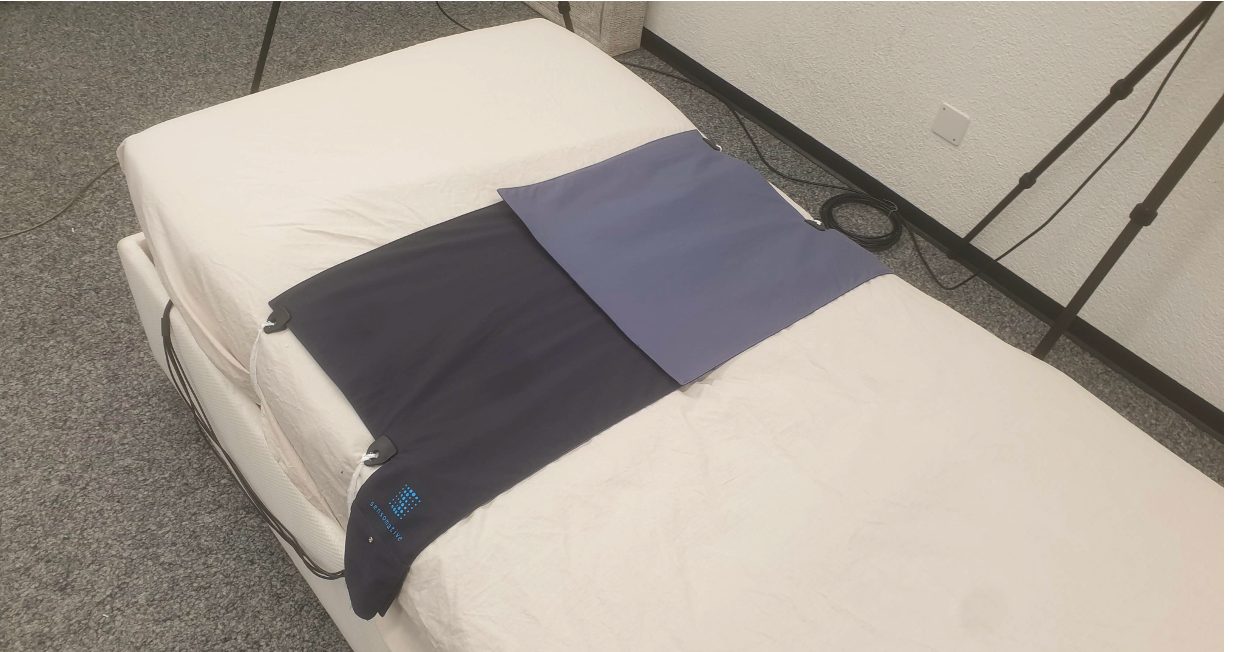
\includegraphics[width=0.9\textwidth]{img/sensomative.png}
    \caption{Sensomative over a bed}
    \label{fig:sensomativeBed}
\end{figure}
\vspace*{0.5cm}

However, its dimension of 40 cm x 80 cm does not allow it to cover the entire mattress so it is crucial to find the correct position to detect the desirable data. In this project, the aim is to estimate the respiration rate so the position chosen is under the lungs, so from just above the shoulder to the middle of the abdomen.

This is to be able to track the movement of the thorax during respiration. The movement is extracted and evaluated from the single sensor channel of the mattress, for the inhalation phase it has been seen an increase in pressure and during the exhalation phase a decrease. Following a pattern [DATA] similar to nasal pressure or RIP Flow, recorded by the cardiopulmonary polysomnography \ref{NOXA1}. 

The data for this mattress are a subsection of the entire data and come from a previous data collection of one of the supervisors of this thesis, Manul Fujis \cite{ManuelZurich}, who kindly make them available to inspect further the possibility to estimate respiratory and hearth rate from this mattress and also to have the data to do a preliminary study of the general feasibility to extract this physiological data. 



\begin{figure}[H]
    \centering
    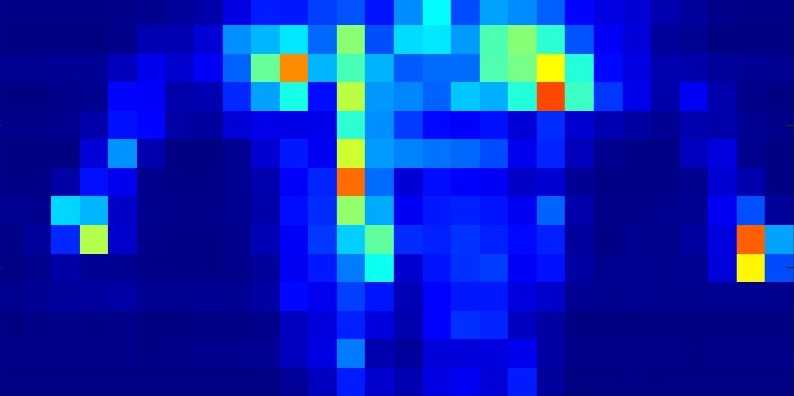
\includegraphics[width=0.9\textwidth]{img/sensomative_2.jpg}
    \caption{Sensomative data}
    \label{fig:sensomativeData}
\end{figure}
\vspace*{0.5cm}

%%%%% SENSINGTEX %%%%%
\subsection{SensingTex} \label{SensigTexPar}
The instrument on which this thesis is focalised then is SensigTex \cite{SensingConnectivity}, visible in Fig \ref{fig:sensingtex} this is a commercially available textile pressure sensor mattress. 
The Mattress Mat Dev Kit is capable to cover the entire area of a bed measuring 192cm x 94cm, with 48 x 22 sensor elements and a sampling rate of 10Hz. This means that is five times slower than Sensomative (Chapter \ref{SensomativePar}), but that is already installed in a hospital ward of the \textit{University of Bern} for the study research on movement disorders during sleep in patients with Parkinson's disease. The ability to estimate breath could be helpful for that study and then this project focused on this possibility.

This mattress is already implemented in the context of position classification, because as shown in Figure \ref{fig:sensingtexData}, is possible to retrieve the position of the person on it. The raw data has is own scale between in range 0-256 (minimum-maximum). 

Looking closer into signals of singles channels is possible to see a pattern that resembles a breathing rhythm,  similar to the data that can
 be retrieved from the nasal pressure exerted on the cannula of cardiorespiratory polysomnography, as shown in Figure \ref{fig:404}.



\vspace*{0.5cm}
\begin{figure}[H]
    \centering
    \includegraphics[width=\textwidth]{img/sensingTex.png}
    \caption{SensigTex over a bed}
    \label{fig:sensingtex}
\end{figure}

\begin{figure}[p]
    \centering
    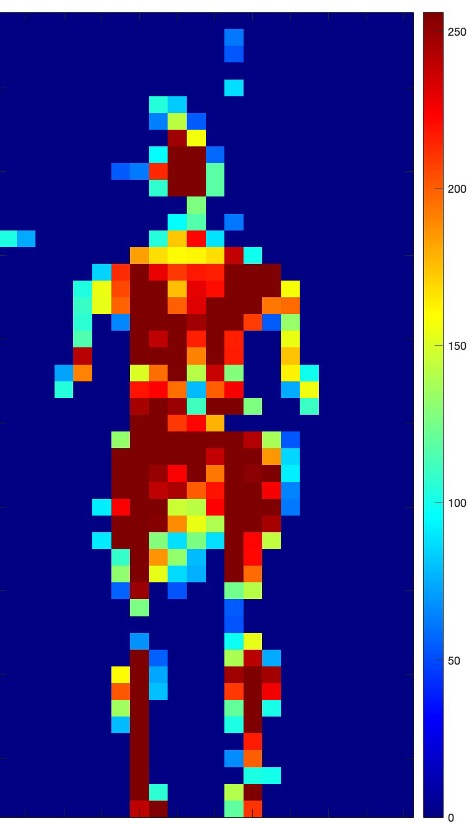
\includegraphics[width=0.7\textwidth]{img/sensingtex_2.jpg}
    \caption{SensigTex Data}
    \label{fig:sensingtexData}
\end{figure}
%\vspace*{0.5cm}

%%%%% NOXA1 %%%%%
\subsection{Nox A1, polysomnography} \label{NOXA1}
As explained in Chapter \ref{cap:cardiorespiratory} the cardiopulmonary polysomnography is an accepted method to monitor physiological data during sleep.

Since in the data collection conducted during the thesis, further explained in Chaper \ref{cap:dataCollection}, it has been necessary to have a gold standard to track respiratory rate and validate estimated respiratory rate from the pipeline, described in Chapter\ref*{cap:pipeline}.

The istrument chosen it has been Nox A1 of NoxMedical, shown in Figure \ref{fig:NOXA1}, a wireless and portable PSG recording the following physiological parameters: 

\begin{itemize}
    \item Nasal pressure and Nasal Flow via nasal cannula.
    \item Chest and Abdomen Movement with respiratory inductance plethysmography (RIP) gathered toghther in a parameter called "RIP Flow"
    \item Heart Rate (ECG)
    \item SPO2 and Pulse with a finger tip
\end{itemize}

In the pipeline (Chapter\ref*{cap:pipeline}) it has been decided to use the Resp Rate (respiratory rate) calculeted by the NOX A1 and displayed as respirations per minute or [rpm] based on RIP Flow data.
However, to further undestand if the channels in the mattress represent the correct respiratory rate are also used Nasal pressure and Nasal Flow.

\begin{figure}[H]
    \centering
    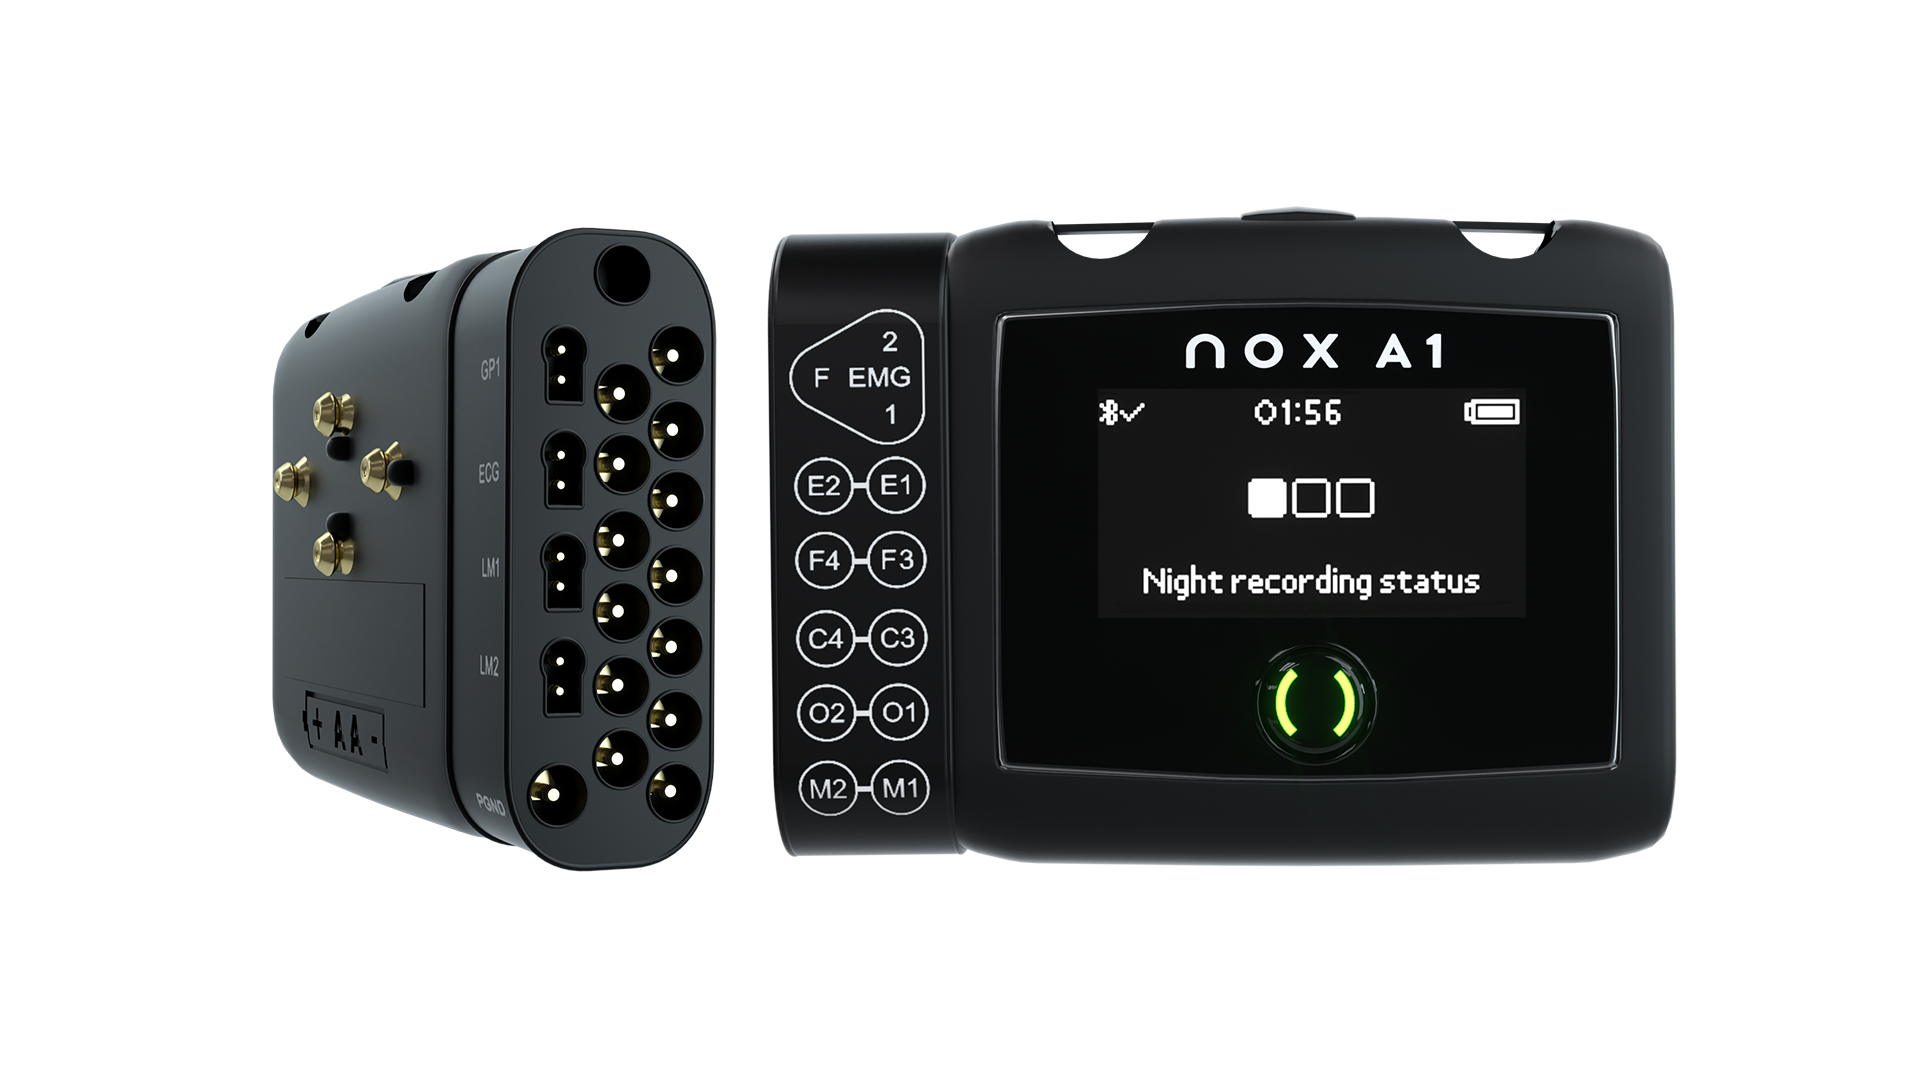
\includegraphics[width=\textwidth]{img/1.png}
    \caption{Nox A1™ PSG System device of NoxMedical}
    \label{fig:NOXA1}
\end{figure}

%%%%% SOMNOMAT %%%%%
\subsection{Somnomat Casa} \label{cap:Somnomat}
The lab, where this thesis is carried out, has one of the main focus on sleep robotics. Inside the Somnomat project, there are two research domain: one covers controlled positional therapy and the other investigates potential benefits of rocking movements on sleep.

The second research domain aim to replicate the rocking movment made from mother to help babies to fall asleep, replicating a back-and-forth motions. The Somnomat Casa, shown in Figure\ref{fig:somnomat}, looks like a conventional bed but fits into private bedrooms and can be operated by the push of a button. 
Rocking movment has determining suitable motion parameters and a mechanical adaptations to have a inaudible rocking mechanism.

The possibility to estimate the respiratory rate of a person while the rocking bed is moving, could be important to discover how this movment could help to fall asleep, based also on the respiration rate. As discussed in Chapter \ref{cap:sleepStages}, breathing is one of the parameter that highlite the sleep stage in which the person is in that moment. This knoledge could be used to further implement the intervention.


\begin{figure}[H]
    \centering
    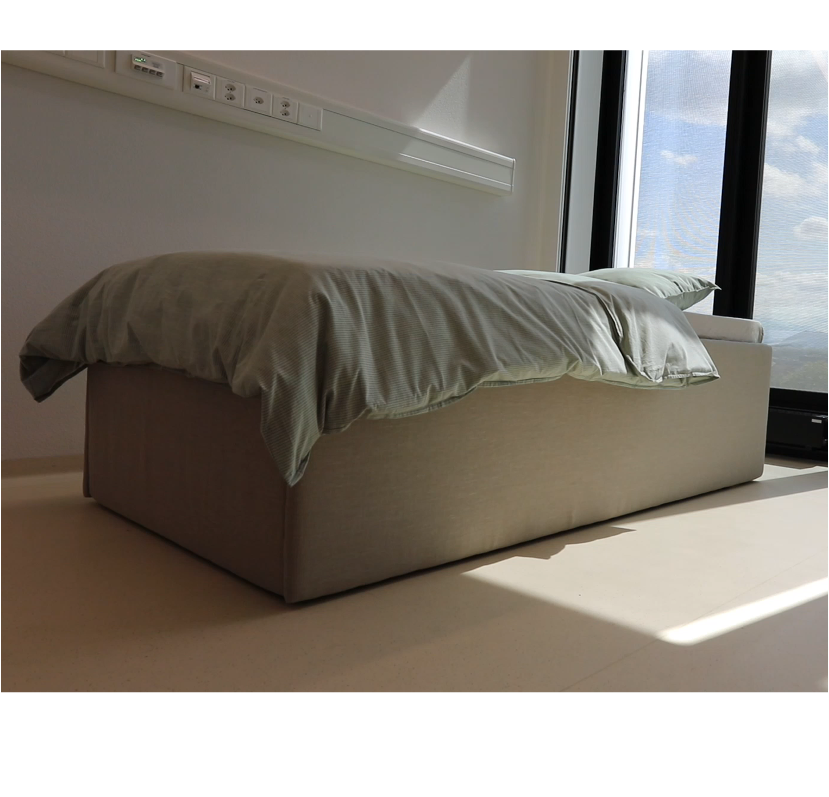
\includegraphics[width=0.8\textwidth]{img/somnomat.png}
    \caption{Somnomat}
    \label{fig:somnomat}
\end{figure}


%%%%% DATA COLLECTION %%%%%
\section{Data Collection} \label{cap:dataCollection}

During the thesis' project has been conducted a data collection because the data from Sensingtex where not has been collected yet.
However, the availability of a rocking bed give to this data collection a second objective.

The primary objective has been to collect data from SensingTex to understand the feasibility of extracting breath rate from the mat; the second goal is to understand if the movement of the rocking bed could influence the signal.\newline

The participant involved was 6, half male and half female, between 20-30 years old, who were asked to lie on a standard mattress covered with the sensor mattresses in a specific position. 
After the 4 minutes, they were asked to turn around in another position following a specific pattern: supine, left side, prone, right side.
Each participant wore a cardiorespiratory wireless and portable polysomnography device (Nox A1 PSG of Nox Medical) that was
monitoring respiratory inductance plethysmography (RIP) which is a method of evaluating pulmonary ventilation by measuring the movement of the chest and abdominal wall, nasal pressure, pulse and heart rate with ECG. 
The study was divided into two phases:
%%%%% NORMAL BED %%%%%
\subsection{Normal Bed}\label{cap:NormalBed}
The setting for the first phase involves the pressure mat over a standard bed. During the night and through the different sleep stages, the breath rate increase or decreases, so we decide to insert a similar variability in our data. We asked the participant to perform a set of five jumps before lying down, so they performed a total of 20 jumps.
%%%%% ROCKING BED %%%%%
\subsection{Rocking Bed}\label{cap:RockingBed}
The setting for the second phase, since in this part we want to collect the data while the Somnomat is moving, we fixed the period for the movement of the bed at 4 seconds (15 periods in a minute) with an acceleration of 0.25 $m/s^2$. Also, for this phase, they have been asked to turn around following the specific pattern: supine, left side, prone, right side.
This results in a recording of 32 minutes long for each participant divided into 4 minutes in each of the 4 positions with normal bed and with Somnomat.


\chapter{Data Analysis}
\section{Weighted and binary method}
\section{Pipeline}
The total number of sensors is 1056, and consequently, the same number of signals from the mattress; this leads to the necessity of an algorithm to discriminate the ones from whom 
it is possible to extract valuable information about the respiratory rate of the person on the mattress.
Many of these channels are stationary on a value; others present just interference from the 
mattress. From just a few sensors, it is possible to retrieve a respiratory pattern and extract the 
respiratory rate per minute (rpm). Therefore becomes necessary to design a metric that underlines these channels.
The meaning of this metric must be interpreted as confidence expressed as the goodness of the signal in percentual.

The designed pipeline aims to replicate a semi-realtime analysis using the data obtained during the data collection. 
For this reason, it takes in input a sliding window of 60 seconds that is moving, for each position, through the 4-minute recording.
The first step excludes those signals for the entire window length that are stationary or present only interference from the mattress.
That interference appears as spikes but sometimes is present just in a percentage of the signal; the same could happen for stationarities that can be focused in just a subpart of the windows. In this case, the signal is not excluded and is assigned with confidence equal to the percentage of the signal that could have meaningful information.
 Another type is a noisy signal, excluded or weighted with a percentage of confidence with the same approach as the previous two.

 After these preliminary analyses, the number of signals decreases drastically; as a result, we obtain signals that could contain valuable information.
We assume to count as one breath the moment between inhale and exhale, which can also be considered a peak in the signal.
At this point, most of the signals are still noisy. To be better analysed, we decide to denoise it (NON SO CHE TERMINE USARE) using 
two different kinds of approaches: Multiresolution analysis of the maximal overlap discrete wavelet transform (hereafter also referred to as "MODWTMRA"), and Savitz-Golay filter.

The MODWTMRA is based on wavelet analysis(MOWDT) that transforms the original signal into a time-frequency domain 
to be analysed and processed, the multiresolution analysis (MRA), which cuts the signal into components, can produce the original signal exactly when added back together.
For our approach, we choose the Daubechies wavelet with two vanishing moments that better represent the breath signal present in our data, so we slide it across the entire signal to vary its location, where we multiply the wavelet and signal at each time step. 
The product of this multiplication gives us a coefficient for that wavelet scale at that time step. 
We then increase the wavelet scale and repeat the process to obtain the signal divided into different scales that combine to recreate the original signal. 
To obtain our denoised signal, we decided to extract and sum only a subset of this scale, which allowed us to reconstruct a clear signal where the peaks could be underlined and counted.

The Savitz-Golay filter, hereafter also referred to as "SG filter", is a filter used to "smooth out" a noisy signal whose frequency span (without noise) is significant. 
They are also called digital smoothing polynomial filters or least-squares smoothing filters. 
The idea of Savitzky-Golay filters is that each sample in the filtered sequence takes its direct neighbourhood of N neighbours and fits a polynomial to it.
So, in the end, is possible to obtain a wave similar to the one in MODWTMRA form, which is likely to count the peaks, interpreted as the rpm.

The so reconstructed signals were given as input to a pick finder to select both peaks and valleys of the signal. 
We then exclude the channels with a signal with more than 30 rpm because the normal rpm during sleep is between 8-25 rpm, but since over 20 is predictive of cardiopulmonary arrest, we decide to keep only signals under 30 rpm.

The remaining signals are further analyzed in their structure: via Euclidean distance between the signal's valley and peaks should differ by up to ±20$\%$ from the preceding breath, and also via the distance between peaks and valleys on the time axis that should vary between ±20 \% from the previous breath.
These two last analysis also gives a percentage of confidence that the signal recreates a breath pattern.

In the end, to calculate the rpm, the channels with the highest accuracy are taken into account, and the rpm is computed as the average of the number of peaks of the signals.
It is also possible to visualize a heatmap to understand where the best channel is in respect of the body. 


\subsection{Excluding criteria}
\subsection{Wavelet}
\subsubsection{theory}
\subsubsection{using in the thesis}
\subsection{Savitz-Golay filter}
\subsubsection{theory}
\subsubsection{using in the thesis}
\subsection{Subsequent analyses of the filtered signal}
\subsection{Result of the Pipeline (visual)}


\chapter{Result}

At the end of the pipeline, has been computed a respiratory rate per minute (rpm), for each position of both conditions (normal bed and rocking bed). This number is obtained as the average of the number of peaks of the channels with the highest confidence that outstrip the value of confidence set as a minimum, at the beginning of the pipeline, to accept the channels (in this case has been 80\%), as discussed in Chapter \ref{cap:computeRespiratory}. 
The following section \ref{cap:metrics} presented the metric used to asset the error between the estimated rpm resulting from the pipeline and the one given by the ground truth. These metrics are commonly employed to determine the difference between medical instruments \cite{Hunt2015IdentificationExercise,HoogAntink2020BallistocardiographyIntervention, Sadek2020AStudy}.
To assert better how the pipeline works, it also shows visually the raw data of the channel with the highest confidence, his reconstruction or filtering and nasal pressure at that moment.

The results are divided into the different combinations of approaches and methods applied to the different positions and conditions.
The result for the following combination can be found in the section:
\begin{itemize}
  \item   Multiresolution Overlap Discrete Wavelet Transform  (MODWTMRA) with binary approach.
  \item  Multiresolution Overlap Discrete Wavelet Transform  (MODWTMRA) with weighted approach
  \item Savitzky–Golay filter with binary approach
  \item  Savitzky–Golay filter with weighted approach   
\end{itemize}



\section{Evaluation Metrics} \label{cap:metrics}
To evaluate the result of the pipeline has been chosen metrics that are on the same scale as the target prediction. This decision has been done to preserve the scale and has an estimation of the difference based on the number of breaths per minute, in our result from the actual value.
The chosen evaluation metrics are: Mean absolute error (MAE), discussed in section \ref{cap:mae} and Mean absolute percentage error (MAPE), discussed in section \ref{cap:mape}. These metrics are usually presented combined with the Bland–Altman plot, further discussed in section \ref{cap:plottino}.


\subsection{Mean absolute error} \label{cap:mae}
Mean Absolute Error (MAE) is the average absolute error between actual and predicted values.  It is a measure of model accuracy given on the same scale as the prediction target, it can be seen as the average error that the model's prediction has in comparison with their corresponding actual targets.

\vspace{0.45cm}

$$MAE = \frac{1}{n} \sum_{i=1}^{n}|y_i-x_i|$$

\vspace{0.45cm}

where $y_i$ is the prediction (pipeline's result), $x_i$ the true value (ground truth respiration rate) and $n$ sample size.

\subsection {Mean absolute percentage error} \label{cap:mape}
Mean Absolute Percentage Error (MAPE) is the mean of all absolute percentage errors between the predicted and actual values.
MAPE is the average percentage difference between predictions and their intended targets in the database.
\vspace{0.45cm}

$$MAPE = \frac{100}{n} \sum_{i=1}^{n}\bigg | \frac{y_i-x_i}{x_i}\bigg |$$ 

\vspace{0.4cm}

where $y_i$ is the prediction (pipeline's result), $x_i$ the true value (ground truth respiration rate) and $n$ sample size. 

 %\subsection{Root Mean Square Error (RMSE) }\label{cap:rmse}
 %Root Mean Squared Error (RMSE) is the square root of the mean squared error between the predicted and actual values.
 %RMSE is a weighted measure of model accuracy given on the same scale as the prediction target. It can be interpreted as the average error that the model’s predictions have in comparison with the actual, with extra weight added to larger prediction errors.
 
 %Abbreviations:
%\begin{itemize}  \item SGf = Savitzky–Golay filter \item resp rate = data extracted from Noxtural   \item toolbox = toolbox for analyzing respiratory recordings %\cite{Noto2018AutomatedToolbox} \end{itemize}


%%%%%% Bland–Altman %%%%%%
\subsection{Bland–Altman Plot} \label{cap:plottino}
The Bland-Altman plot is highly employed in medical statistics to visualize the difference in measurements between two different instruments or two different measurement techniques. An example is shown in Figure \ref{fig:exxampleBland}.

\vspace{1cm}
\begin{figure}[H]
  \centering
  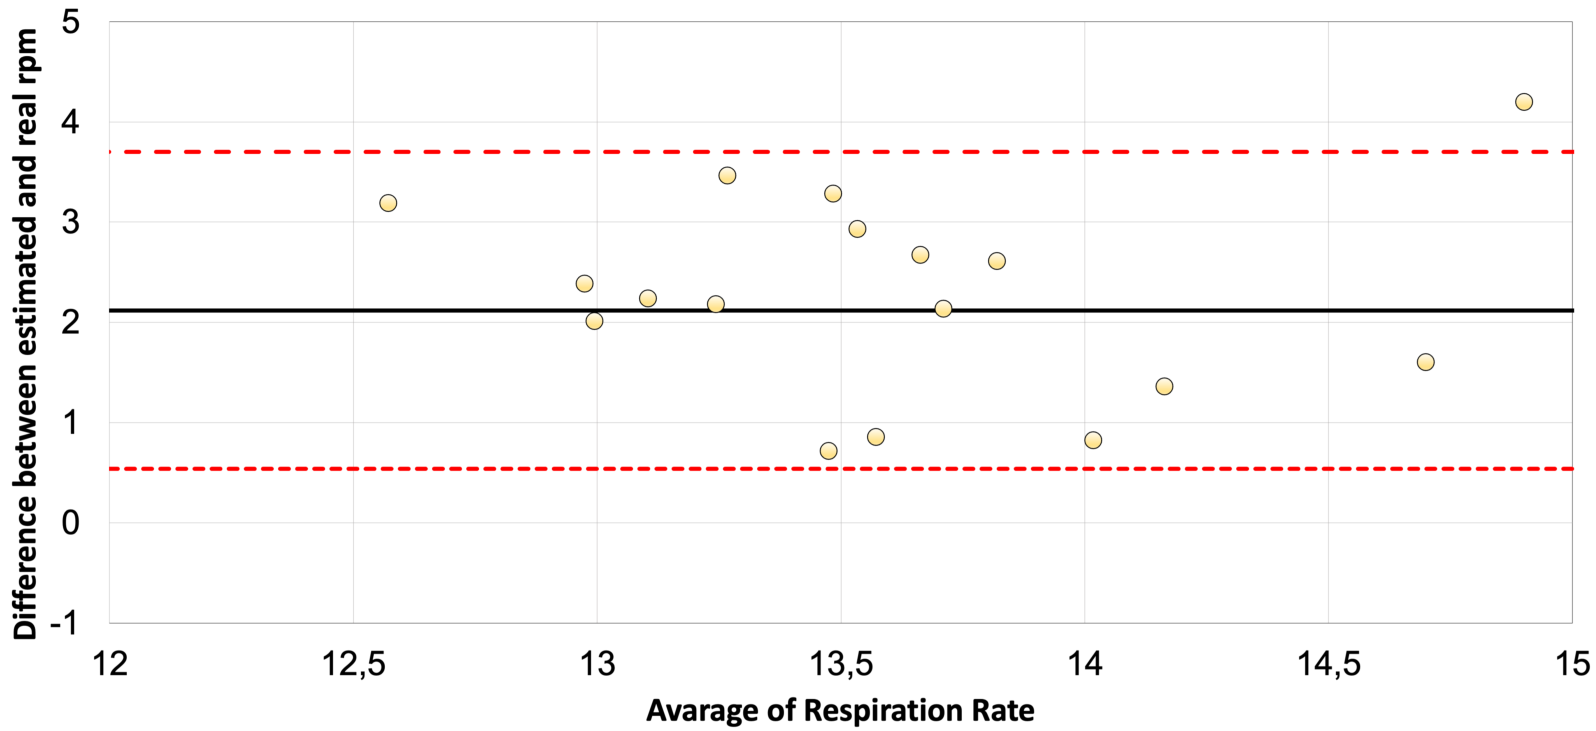
\includegraphics[width=\textwidth]{img/balnd1.pdf}
  \caption{Example of Bland Altman Plot}
  \label{fig:exxampleBland}
\end{figure}
\vspace{1cm}

The \textit{x-axis} of the plot displays the average measurement of the two instruments and the \textit{y-axis} displays the difference in measurements between the two instruments. In the plot are present also three lines, the central black represents the average difference in measurements between the two instruments also known as ``bias'' between the two measurements, as far from zero as large the average difference is large. The red dotted lines are the limits of the agreement, defined as the mean difference $\pm 1.96$ standard deviation of the difference. 




\clearpage
%%%%%% MODWTMRA %%%%%%
\section{Result for MODWTMRA} \label{cap:ResultMODWTRA}


This section of the result is divided into normal bed, section \ref{cap:ResultNormalBed1}, and rocking bed \ref{cap:ResultRockingBed1}. Inside both sections are presented the result for each position for the binary and weighted approach, the denoise method is MODWTMRA.

The estimated respiratory rate per minute (rpm) while the participants are on the mattressare further presented. Given the use of a moving window to simulate a real-time pipeline, the estimated rpm for each window is shown. 
The total number of windows for each position is 18 since the window is 60 seconds long and the entire recording for each position is 4 minutes long. 
First, is presented the table containing the estimated rpm using binary and weighted approaches compared with the rpm given by the ground truth. 
After is shown a table with the average rpm for both approaches and the relative mean absolute error (MAE) and mean absolute percentage error (MAPE). In the end, are presented the Bland–Altman plot to better visualize and understand the data in respect of the error and a plot of the best channel with its raw data and relative denoised wave.


%%%%%% NORMAL BED %%%%%%
\subsection{Normal Bed}

The participant in this phase has to perform a series of jumps before lying on the mattress due to recreating the increase or decrease of the breath rate between the different sleep stages. This phase aims to understand the feasibility of extracting breath rate from the mat. For this phase, the mattress is placed on a standard bed.

%%%%%% NORMAL BED - SUPINE %%%%%%

\subsubsection{Result Normal Bed in Supine Position}   \label{cap:ResultNormalBed1}

The estimated respiratory rate per minute (rpm) while the participants are supine with the mattress placed on a normal bed is further presented. Table \ref{tab:SupineNormalStill} presented the estimated rpm using binary and weighted approach compared with the rpm given by the ground truth. The approaches retrieve an almost identical rpm, this result may be due to the choice of the minimum confidence value at 80\% that allows keeping only the best signal, maybe with higher confidence can be seen a higher difference between the two approaches. 

\vspace{0.5cm}
\begin{table}[h]
    \centering
    \begin{tabular}{|c|c|c|}
    \hline 
     Binary  &  Weighted & RPM (NOXA1)  \\%& toolbox \\ 

    \hline 
     14.8438  & 14.7353  & 13.485 \\ % & 14 \\ %
   14  & 14  & 13.1443 \\%& 13 \\ 
     15.125  & 15.125 & 12.5154 \\ %& 13 \\ 
    13.8333  & 13.8333 &13.117\\ % & 13 \\ 
  14.4286  & 14.4286 & 13.6077\\ % & 14 \\ 
    15.5  & 15.5 & 13.8993\\ %& 15 \\ 
     15 &  15 & 12.0681\\ % & 15 \\ 
  11 &  11 & 11.4768\\ % & 15 \\ 
 14.3333 &  14.3333 & 12.1549 \\ %& 14 \\ 
  17 &  17 & 12.8028 \\ %& 13 \\ 
 15 &  15 & 12.3275 \\ %& 14 \\ 
 14.1667 & 14.1667 & 10.9785 \\ %& 11 \\ 
  15.125 & 15.125 & 11.8441 \\ %& 11 \\ 
 14.7778 &  14.7778 & 12.6438\\ % & 10 \\ 
    15 &  15 & 11.5351 \\ %& 11 \\ 
    14 & 14 & 11.99 \\ %& 10 \\ 
    14.2222 & 14.2222 & 11.9868 \\ %& 10 \\ 
    14.1667 &  13.8571 & 11.7824 \\ %& 10 \\ 

    \hline 
    \end{tabular}
    \caption{Estimated rpm using binary and weighted approach of the pipeline compared with the rpm given by the ground truth - Normal bed and supine position}
    \label{tab:SupineNormalStill}
\end{table}





 
    

Table \ref{tab:SupineNormalStillMetrics} present the average rpm for both approaches  
and the relative mean absolute error (MAE) and mean absolute percentage error (MAPE). As just discussed in the previous paragraph there is no substantial difference between the two different approaches. The data on which to focus more is the number of breaths that the algorithm misses, represented by MAE and expressed in percentage by MAPE. The average number is 2rpm, which means that if we consider the estimated average of 14.5rpm the error is almost 20\%, quite high for an approach that must be used in the medical field.

%\vspace{0.5cm}
\begin{table}[H]

    \centering
    \begin{tabular}{|c|c|c|}
    \hline 
    & Binary  & Weighted  \\ 
    \hline 
    rpm mean & 14.529 &  14.506\\
    MAE rpm  & 2.1731  &  2.1499 \\ 
    MAPE  & 17.8104\%  & 17.6198\% \\ 
    \hline 
    \end{tabular}
    
    \caption{Avarage number of breath for each approach with the relative mean absolute error (MAE) and mean absolute percentage error (MAE) - Normal bed and supine position}
    \label{tab:SupineNormalStillMetrics}
\end{table}

Figure \ref{fig:baln1} show the Bland–Altman plot, presented in section \ref{cap:plottino}, of the estimated rpm from the pipeline compared to the value of the ground truth. It helps to visualize the data from Table \ref{tab:SupineNormalStillMetrics} in respect of the error. Since the result for the approaches is similar the data presented with this plot refers to the weighted approach only.

Figure \ref{fig:rec} shows the denoised signal using MODWTMRA with the highest accuracy (92\%) for the supine position with a normal mattress.

\begin{figure}[p]
  \centering
  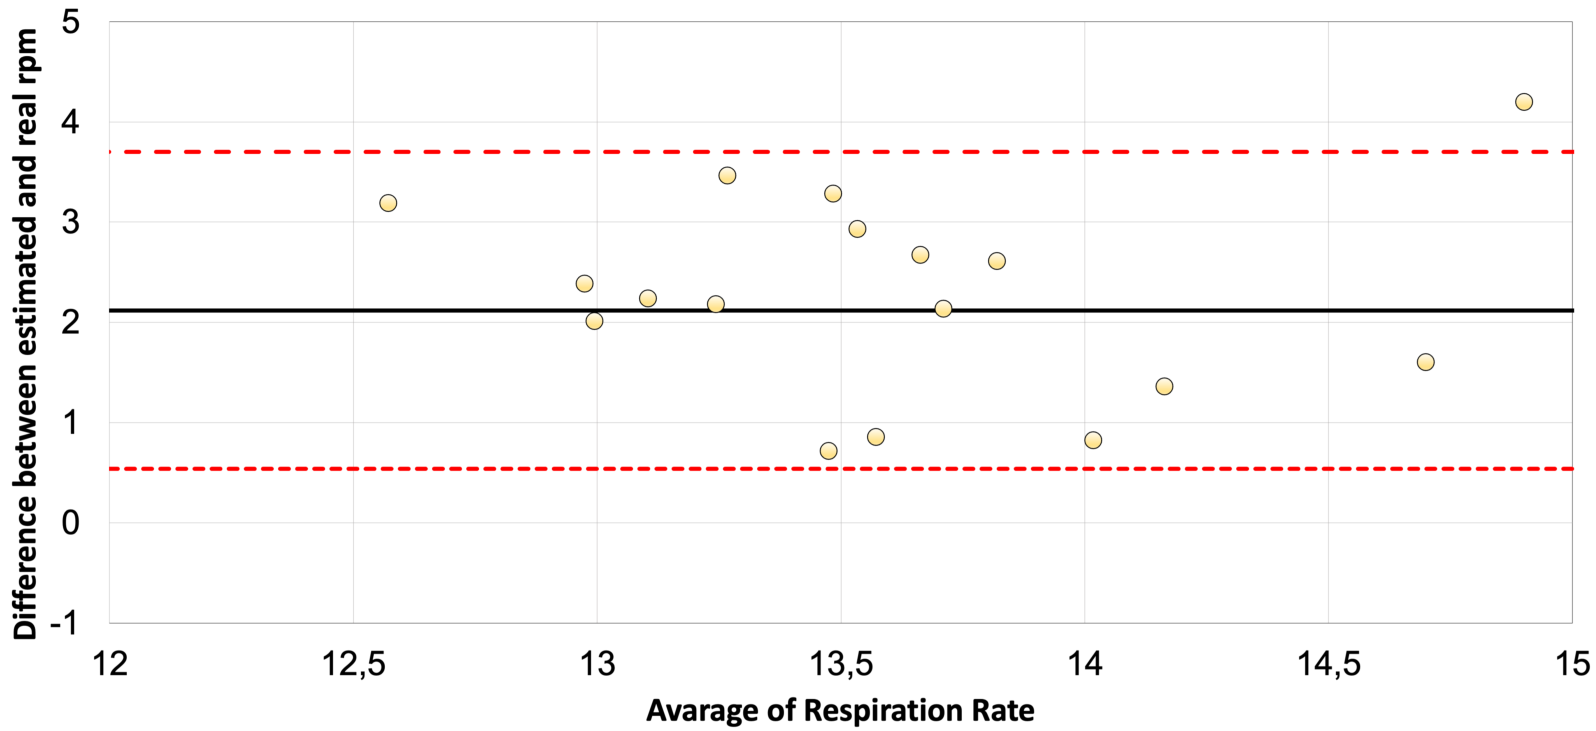
\includegraphics[width=\textwidth]{img/balnd1.pdf}

  \caption{Bland Altman Plot of estimated rpm from the pipeline compared to the value of the ground truth - Normal bed and supine position}
  \label{fig:baln1}
  \vspace{1.5cm}
  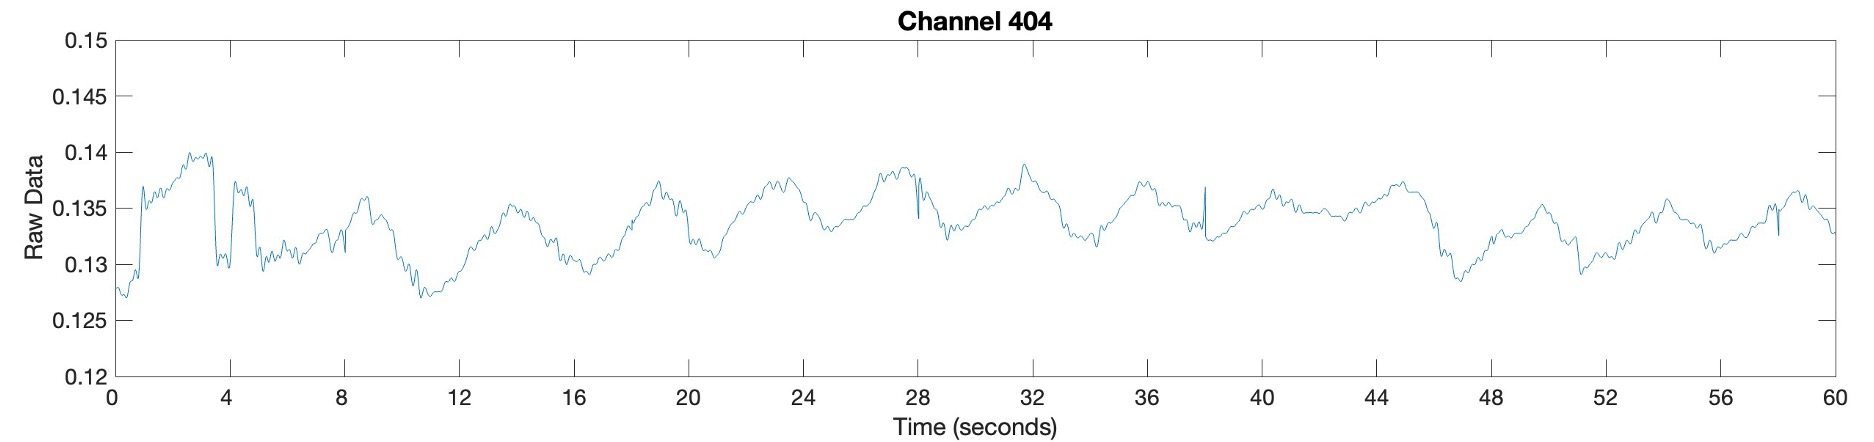
\includegraphics[width=\textwidth]{img/404.jpg}
  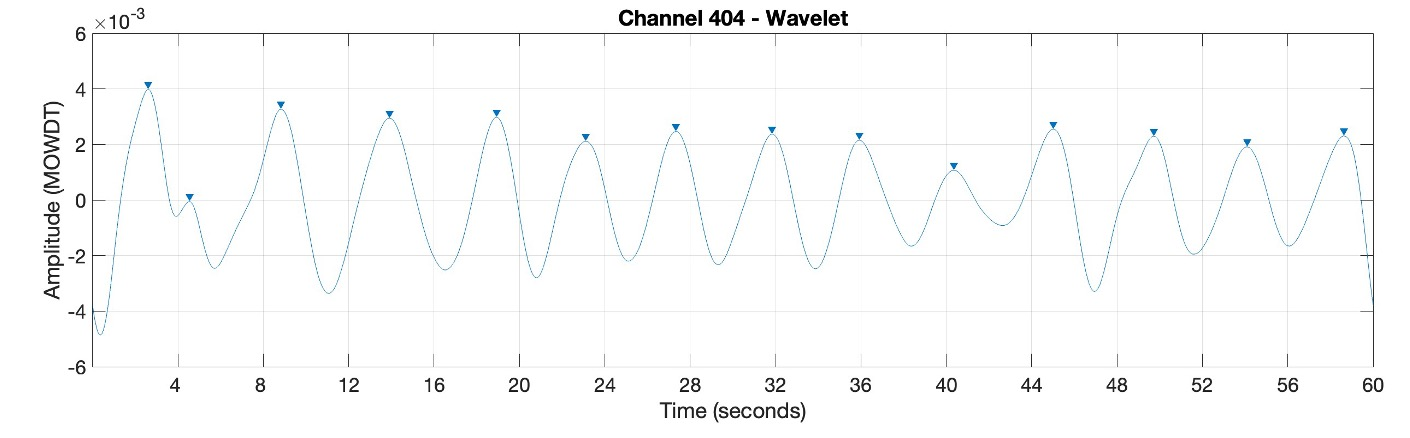
\includegraphics[width=\textwidth]{img/404_wave.jpg}
\caption{Raw data and denoised signal using MODWTMRA of the channel with the highest percentage of confidence (92\%) - Normal bed and supine position}
  \label{fig:rec}
\end{figure}


\clearpage
%%%%%% Rocking  Bed %%%%%%
\subsection{Rocking Bed}
The second part of the data collection aims to understand if the movement of the
rocking bed could influence the signal. The participant has to lie on the mattress without jumps, to have less variability in the data. For this phase, the mattress is placed on a rocking bed, which periods have been fixed at 4 seconds (15 periods in a minute) with an acceleration of 0.25 $m/s^2$.


%%%%%% Rocking BED - SUPINE %%%%%%

\subsubsection{Result Rocking Bed in Supine Position}  % \label{cap:ResultNormalBed1}

The estimated respiratory rate per minute (rpm) while the participants are supine with the mattress placed on a rocking bed is further presented. 

Table \ref{tab:SupineMov} presented the estimated rpm using binary and weighted approach compared with the rpm given by the ground truth. The approaches retrieve an almost identical rpm. 

\vspace{0.5cm}
\begin{table}[H]
    \centering
    \begin{tabular}{|c|c|c|}
    \hline 
    Binary & Weighed  & RPM (NOXA1) \\ 
    \hline
15.5       &  15.5    &  10.7609 \\ 
16.1333     & 16.1333  &    11.3077 \\ 
15.3333    &  15.3333   &   13.1449 \\ 
14.9474    &  14.9474    &  11.3366 \\ 
15.1       &  15.1     & 12.7314 \\ 
15.6364   &   15.6364   &   11.8892 \\ 
14.6923    &  14.6923    &    11.42 \\ 
15.2222    &  15.2222    &  13.0092 \\ 
15.1667    &  15.1667    &  13.2539 \\ 
14.6667    &  14.6667    &  11.6391 \\ 
15         &  15    &  12.2165 \\ 
14.75       & 14.75  &    11.9216 \\ 
15           &15    &  11.3091 \\ 
14.625    &   14.625   &   13.8905 \\ 
15.6154    &  15.6154   &   11.3344 \\ 
15   &   14.8182   &   11.4474 \\ 
15.1765   &   15.1765   &   11.6675 \\ 
14.6154  &    14.6154    &  13.4799 \\
\hline 
    \end{tabular}
\caption{Estimated rpm using binary and weighted approach of the pipeline compared with the rpm given by the ground truth - Rocking bed and supine position}
\label{tab:SupineMov}
\end{table}

Table \ref{tab:SupineMov} present the average rpm for both approaches  
and the relative mean absolute error (MAE) and mean absolute percentage error (MAPE). As just discussed in the previous paragraph there is no substantial difference between the two different approaches. The data on which to focus more is the number of breaths that the algorithm misses, represented by MAE and expressed in percentage by MAPE. The average number is 3rpm, which means that if we consider the estimated average of 15.1rpm the error is almost 25\%, is too high for an approach that must be used in the medical field.

%\vspace{0.5cm}

\begin{table}[h]

    \centering

\begin{tabular}{|c|c|c|c|c|}
\hline 
& Binary & Weighed \\ 
 
\hline 
rpm mean & 15.1211  & 15.1110 \\  
MAE resp   & 3.0234 &     3.0133 \\ 
MAPE resp  & 25.7324\% &  25.6442\% \\ 

\hline 
\end{tabular}
\caption{Evarage number of breath for each approach with the relative mean
absolute error (MAE) and mean absolute percentage error (MAE) - Rocking bed
and right side}
\label{tab:SupineRockingMetrics}
\end{table}

Figure \ref{fig:baln1} show the Bland–Altman plot, presented in section \ref{cap:plottino}, of the estimated rpm from the pipeline compared to the value of the ground truth. It helps to visualize the data from Table \ref{tab:SupineRockingMetrics} in respect of the error. Since the result for the approaches is similar the data presented with this plot refers to the weighted approach only.

Figure \ref{fig:rec} shows the denoised signal using MODWTMRA with the highest accuracy (92\%) for the supine position with a normal mattress.

\begin{figure}[p]
  \centering
  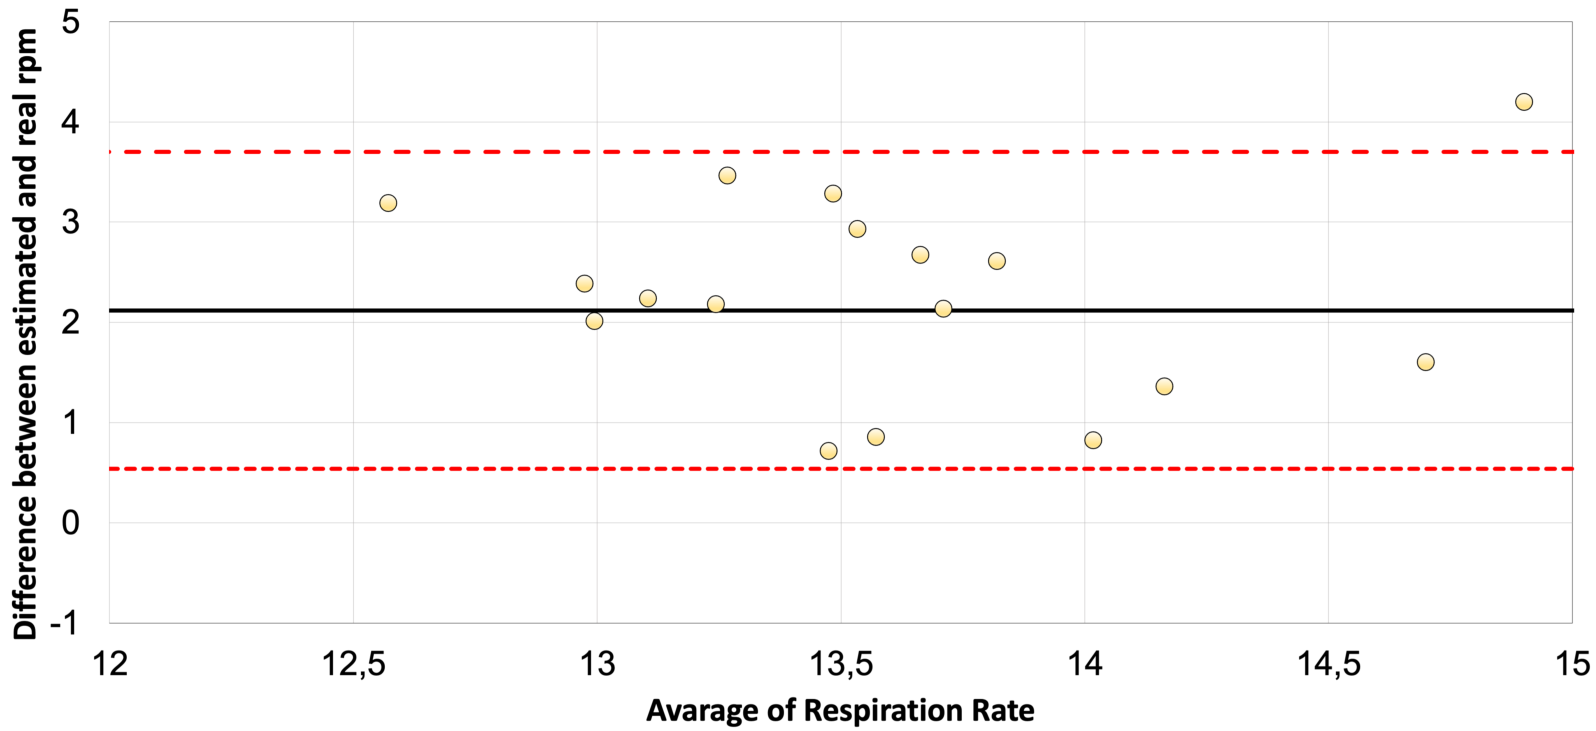
\includegraphics[width=\textwidth]{img/balnd1.pdf}

  \caption{Bland Altman Plot of estimated rpm from the pipeline compared to the value of the ground truth - Rocking bed and supine position}
  \label{fig:baln1}
  \vspace{1.5cm}
  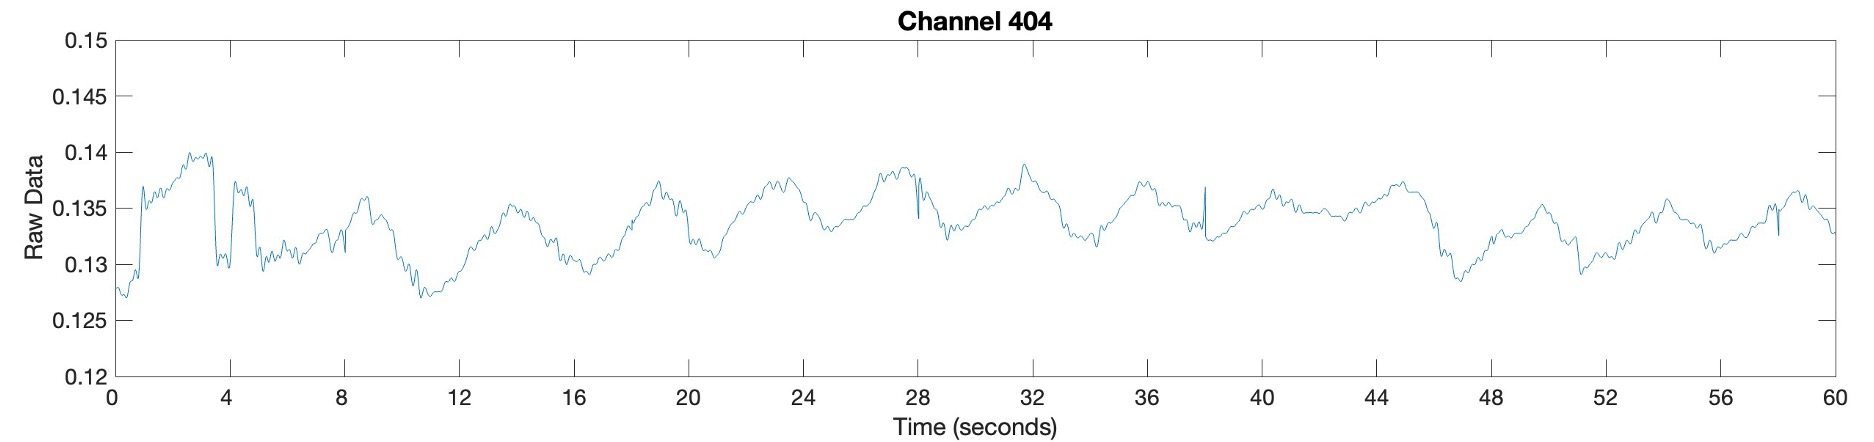
\includegraphics[width=\textwidth]{img/404.jpg}
  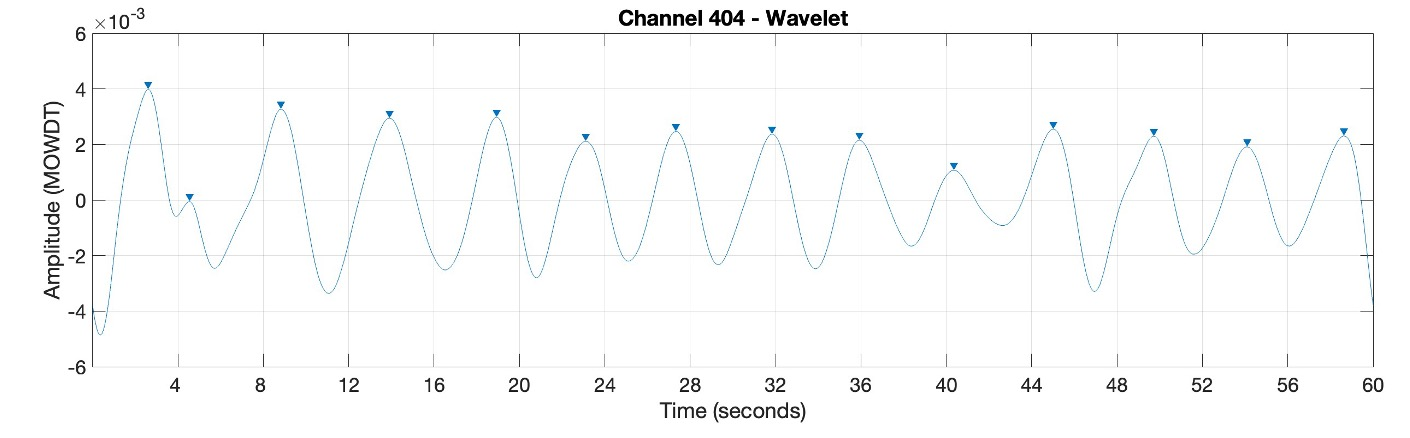
\includegraphics[width=\textwidth]{img/404_wave.jpg}
\caption{Raw data and denoised signal using MODWTMRA of the channel with the highest percentage of confidence (92\%) - Normal bed and supine position}
  \label{fig:rec}
\end{figure}



%%%%%% FILTRO %%%%%%
\section{Result for Savitzky–Golay filter} \label{cap:ResultSG}

The result presented in this section are denoised with Savitzky–Golay filter and are
 divided into normal bed, section \ref{cap:normalSavitz}, and rocking bed \ref{cap:RockSavitx}. Inside both sections are presented the result for each position for the binary and weighted approach.


%%%%%% NORMAL BED %%%%%%
\subsection{Normal Bed} \label{cap:normalSavitz}

The participant in this phase has to perform a series of jumps before lying on the mattress due to recreating the increase or decrease of the breath rate between the different sleep stages. This phase aims to understand the feasibility of extracting breath rate from the mat. For this phase, the mattress is placed on a standard bed.

%%%%%% NORMAL BED - SUPINE %%%%%%

\subsubsection{Result Normal Bed in Supine Position}  
The estimated respiratory rate per minute (rpm) while the participants are supine with the mattress placed on a normal bed is further presented. Table \ref{tab:SupineNormalStillsg} presented the estimated rpm using binary and weighted approach compared with the rpm given by the ground truth. The approaches retrieve an almost identical rpm, this result may be due to the choice of the minimum confidence value at 80\% that allows keeping only the best signal, maybe with higher confidence can be seen a higher difference between the two approaches. 

\vspace{0.5cm}
\begin{table}[h]
    \centering
    \begin{tabular}{|c|c|c|}
 
    \hline 
    Binary & Weighed & RPM (NOXA1) \\ 
    \hline 
    12.8529  & 12.8333  & 13.485  \\ 
    12.0909  & 12.0909  & 13.1443  \\ 
    11.9167  & 11.9167  & 12.5154  \\ 
    13.3333  & 13.4  & 13.117  \\ 
    12.2857  & 12.2857  & 13.6077 \\ 
    12.5833  & 12.3077  & 13.8993 \\ 
    11.6  & 11.6 & 12.0681  \\ 
    9 &  9  & 11.4768  \\ 
    11.1667  & 10.625  & 12.1549  \\ 
    14.5 & 14.5  & 12.8028 \\ 
    14.3333  & 14.3333  & 12.3275  \\ 
    11.625  & 11.625  & 10.9785  \\ 
    13.125  & 13.125  & 11.8441  \\ 
    13.1111  & 13.1111  & 12.6438  \\ 
    13.3077  & 13.3077  & 11.5351  \\ 
    13.6667  & 13.6667  & 11.99  \\ 
    11.5  & 11.5  & 11.9868 \\ 
    11.4545  & 11.2308  & 11.7824 \\ 
    \hline 
\end{tabular}
\caption{Estimated rpm using binary and weighted approach of the pipeline
compared with the rpm given by the ground truth
- Normal bed and supine position}
\label{tab:SupineNormalStillsg}

\end{table}

Table \ref{tab:SupineNormalStillMetricssg} present the average rpm for both approaches  
and the relative mean absolute error (MAE) and mean absolute percentage error (MAPE). As just discussed in the previous paragraph there is no substantial difference between the two different approaches. The data on which to focus more is the number of breaths that the algorithm misses, represented by MAE and expressed in percentage by MAPE. The average number is 2rpm, which means that if we consider the estimated average of 14.5rpm the error is almost 20\%, quite high for an approach that must be used in the medical field.

%\vspace{0.5cm}
\begin{table}[h]
    \centering
    \begin{tabular}{|c|c|c|}
    \hline 
    & Binary SGf & binary Waveleft & weighed  SGf & weighed Waveleft \\ 
    \hline 
    rpm mean &    \\ 
    MAE resp & 1.0796 &       1.1422  \\ 
    MAPE resp & 8.7793 \%  & 9.2789 \% \\ 
    \hline 
    \end{tabular}
    
    \caption{Evarage number of breath for each approach with the relative mean
    absolute error (MAE) and mean absolute percentage error (MAE) - Normal bed
    and supine position}
    \label{tab:SupineNormalStillMetricssg}    
\end{table}
    
    

Figure \ref{fig:baln1} show the Bland–Altman plot, presented in section \ref{cap:plottino}, of the estimated rpm from the pipeline compared to the value of the ground truth. It helps to visualize the data from Table \ref{tab:SupineNormalStillMetricssg} in respect of the error. Since the result for the approaches is similar the data presented with this plot refers to the weighted approach only.

Figure \ref{fig:rec} shows the denoised signal using MODWTMRA with the highest accuracy (92\%) for the supine position with a normal mattress.

\begin{figure}[p]
  \centering
  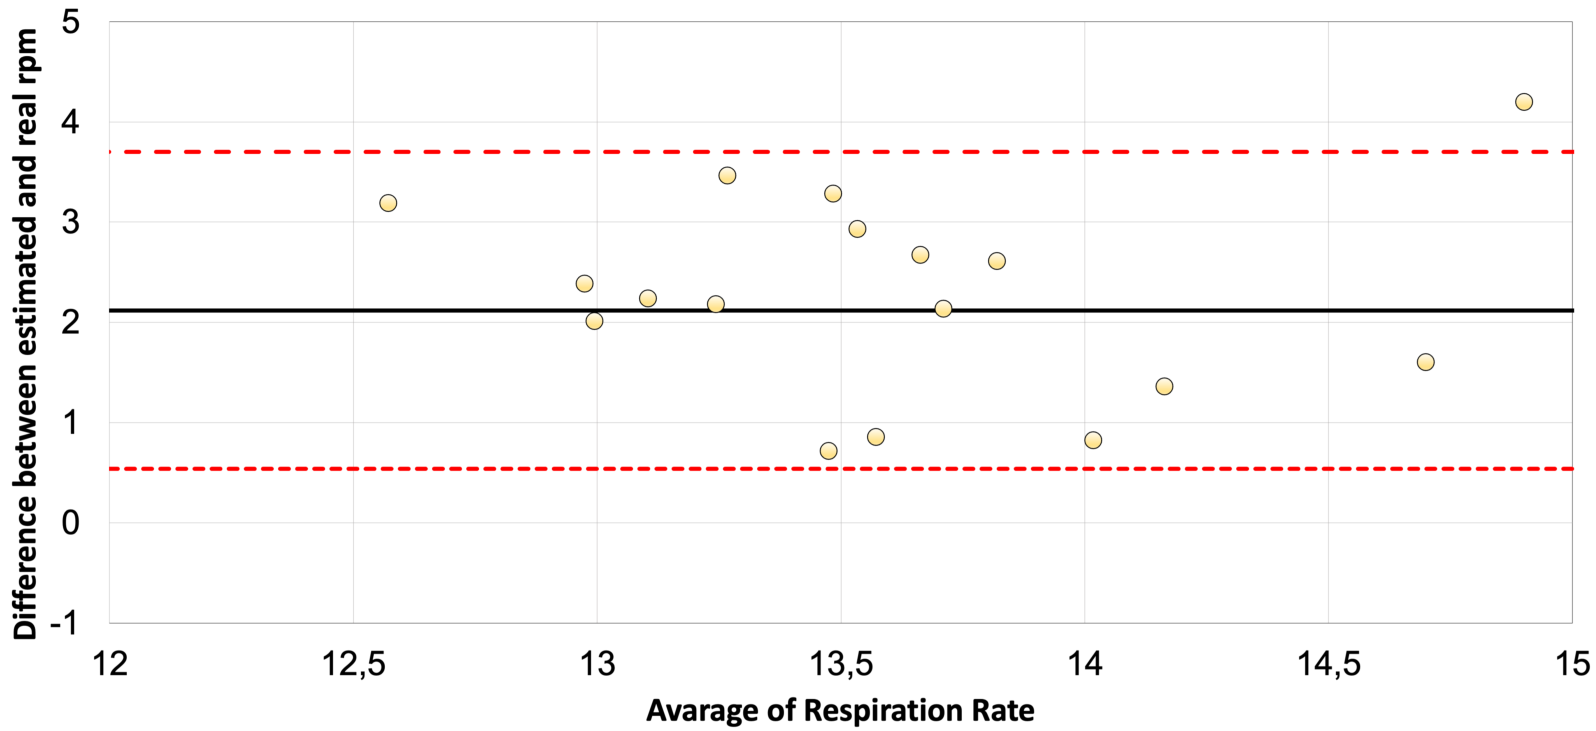
\includegraphics[width=\textwidth]{img/balnd1.pdf}

  \caption{Bland Altman Plot of estimated rpm from the pipeline compared to the value of the ground truth - Normal bed and supine position}
  \label{fig:baln1}
  \vspace{1.5cm}
  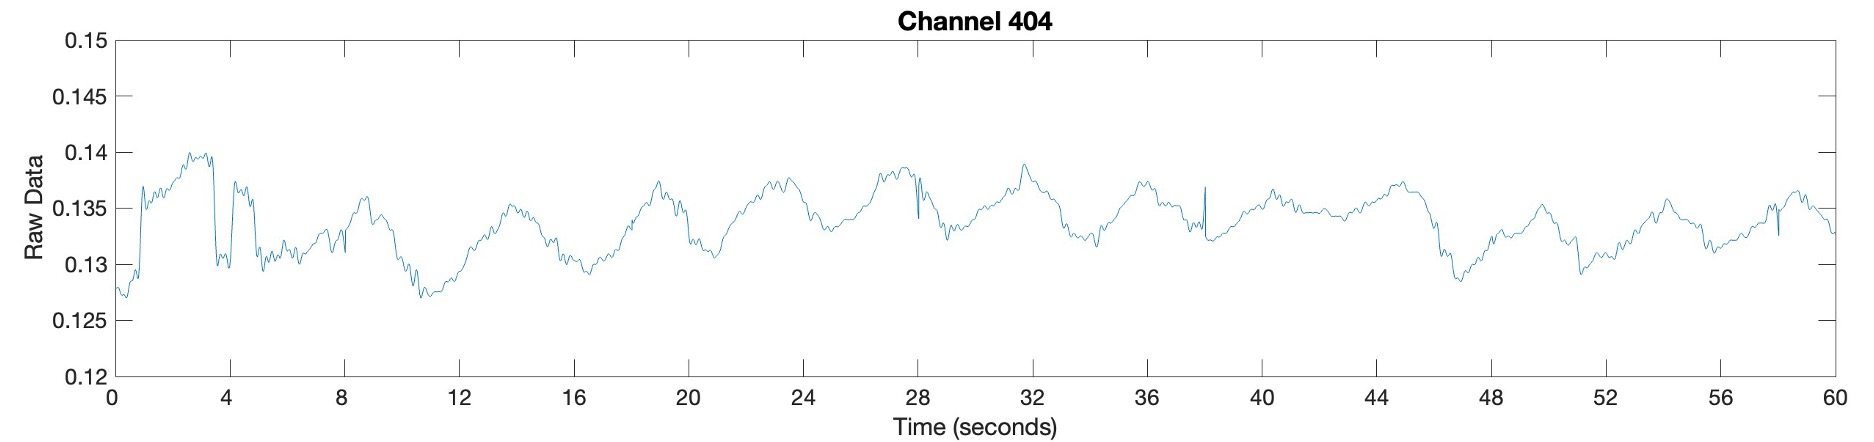
\includegraphics[width=\textwidth]{img/404.jpg}
  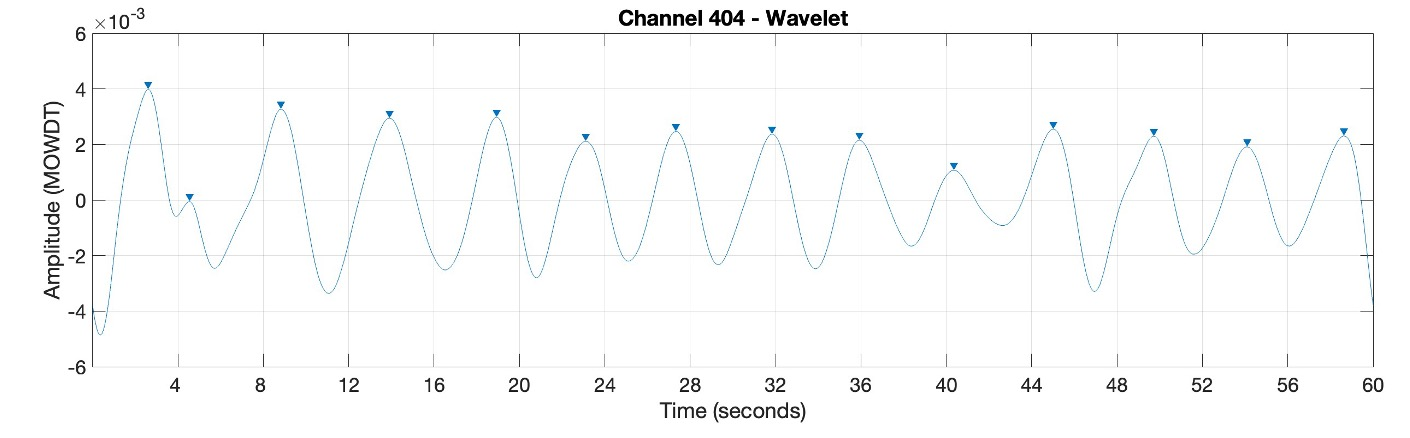
\includegraphics[width=\textwidth]{img/404_wave.jpg}
\caption{Raw data and denoised signal using MODWTMRA of the channel with the highest percentage of confidence (92\%) - Normal bed and supine position}
  \label{fig:rec}
\end{figure}


\clearpage
%%%%%% Rocking  Bed %%%%%%
\subsection{Rocking Bed}\label{cap:RockSavitx}
The second part of the data collection aims to understand if the movement of the
rocking bed could influence the signal. The participant has to lie on the mattress without jumps, to have less variability in the data. For this phase, the mattress is placed on a rocking bed, which periods have been fixed at 4 seconds (15 periods in a minute) with an acceleration of 0.25 $m/s^2$.


%%%%%% Rocking BED - SUPINE %%%%%%

\subsubsection{Result Rocking Bed in Supine Position}  % \label{cap:ResultNormalBed1}

The estimated respiratory rate per minute (rpm) while the participants are supine with the mattress placed on a rocking bed is further presented. 

Table \ref{tab:SupineMovsg} presented the estimated rpm using binary and weighted approach compared with the rpm given by the ground truth. The approaches retrieve an almost identical rpm. 

\vspace{0.5cm}
\begin{table}[h]
    \centering
    \begin{tabular}{|c|c|c|}
 
    \hline 
    Binary & Weighed & RPM (NOXA1) \\ 
    \hline 
14.1667     &  14.1667  &     10.7609 \\ 
14.0667   &    14.0667  &     11.3077 \\ 
13.5     &     13.5  &     13.1449 \\ 
13.75    &     13.75   &    11.3366 \\ 
12.9474    &   12.9474 &      12.7314 \\ 
12.4615   &    12.4615    &   11.8892 \\ 
12.6875   &    12.6875     &    11.42 \\ 
13.5   &    13.6364 &      13.0092 \\ 
14.6154  &     14.6154  &     13.2539 \\ 
13.1429   &    13.1429  &     11.6391 \\ 
14.375   &     14.375  &     12.2165 \\ 
15.4286   &    15.4286   &    11.9216 \\ 
14.6667   &    14.6667   &    11.3091 \\ 
14.8182   &    14.8182   &    13.8905 \\ 
14.5385   &    14.5385  &     11.3344 \\ 
13.9091    &   13.9167  &     11.4474 \\ 
13.8824  &     13.8824  &     11.6675 \\ 
13.8667   &    13.8667   &    13.4799 \\ 
\hline
    \end{tabular}
\caption{Estimated rpm using binary and weighted approach of the pipeline compared with the rpm given by the ground truth - Rocking bed and supine position}
\label{tab:SupineMovsg}

\end{table}

Table \ref{tab:SupineMovsg} present the average rpm for both approaches  
and the relative mean absolute error (MAE) and mean absolute percentage error (MAPE). As just discussed in the previous paragraph there is no substantial difference between the two different approaches. The data on which to focus more is the number of breaths that the algorithm misses, represented by MAE and expressed in percentage by MAPE. The average number is 3rpm, which means that if we consider the estimated average of 15.1rpm the error is almost 25\%, is too high for an approach that must be used in the medical field.

%\vspace{0.5cm}

\begin{table}[h]

    \centering

\begin{tabular}{|c|c|c|c|c|}
\hline 
& Binary & Weighed \\ 
 
\hline 
rpm mean & 13.9068 &  13.9148  \\  
MAE rpm   &  1.8091&      1.8171 \\ 
MAPE   & 15.5385\% &  15.6004\% \\ 

\hline 
\end{tabular}
\caption{Evarage number of breath for each approach with the relative mean
absolute error (MAE) and mean absolute percentage error (MAE) - Rocking bed
and supine position}
\label{tab:SupineRockingMetricssg}
\end{table}

Figure \ref{fig:baln1} show the Bland–Altman plot, presented in section \ref{cap:plottino}, of the estimated rpm from the pipeline compared to the value of the ground truth. It helps to visualize the data from Table \ref{tab:SupineRockingMetricssg} in respect of the error. Since the result for the approaches is similar the data presented with this plot refers to the weighted approach only.

Figure \ref{fig:rec} shows the denoised signal using MODWTMRA with the highest accuracy (92\%) for the supine position with a normal mattress.

\begin{figure}[p]
  \centering
  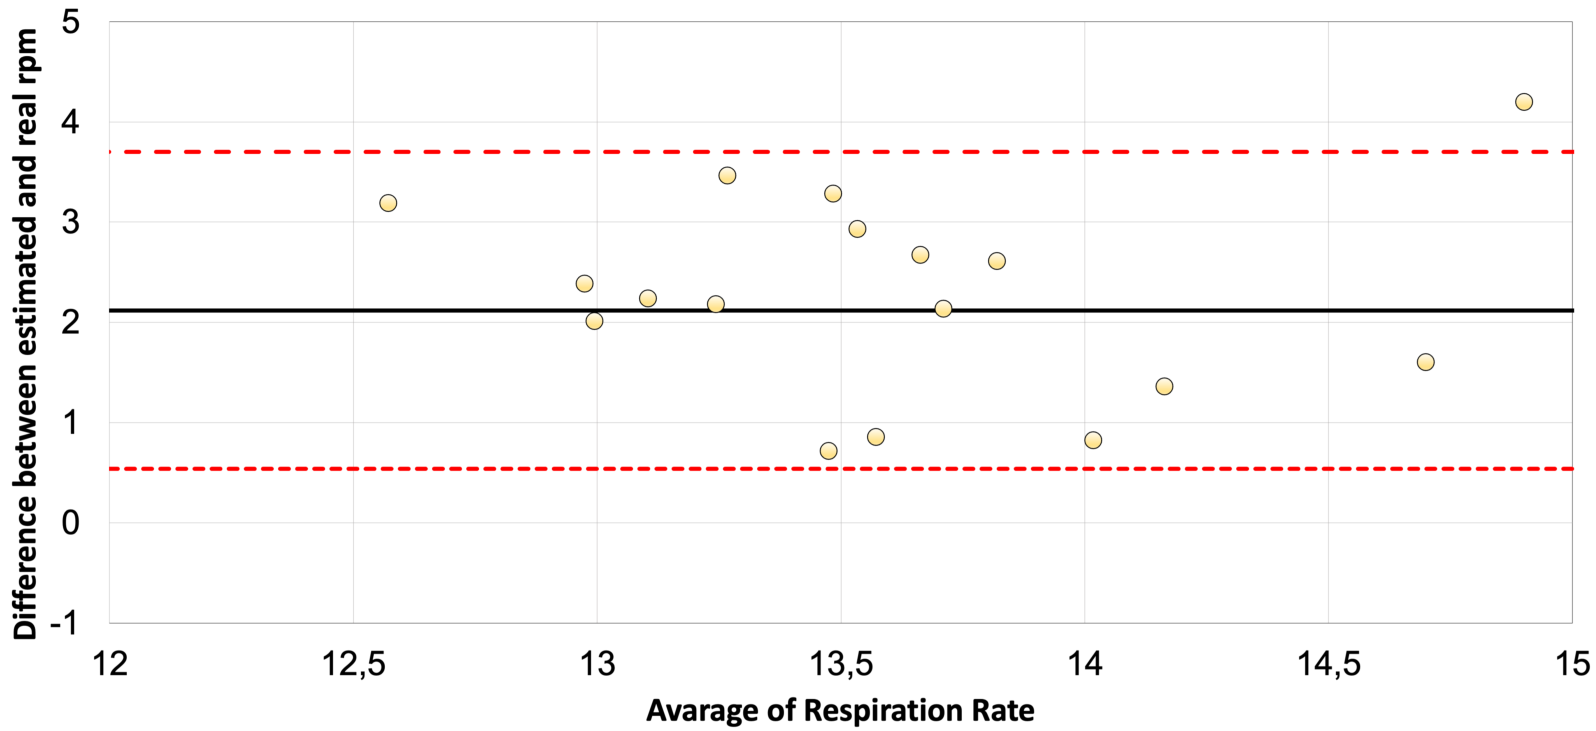
\includegraphics[width=\textwidth]{img/balnd1.pdf}

  \caption{Bland Altman Plot of estimated rpm from the pipeline compared to the value of the ground truth - Rocking bed and supine position}
  \label{fig:baln1}
  \vspace{1.5cm}
  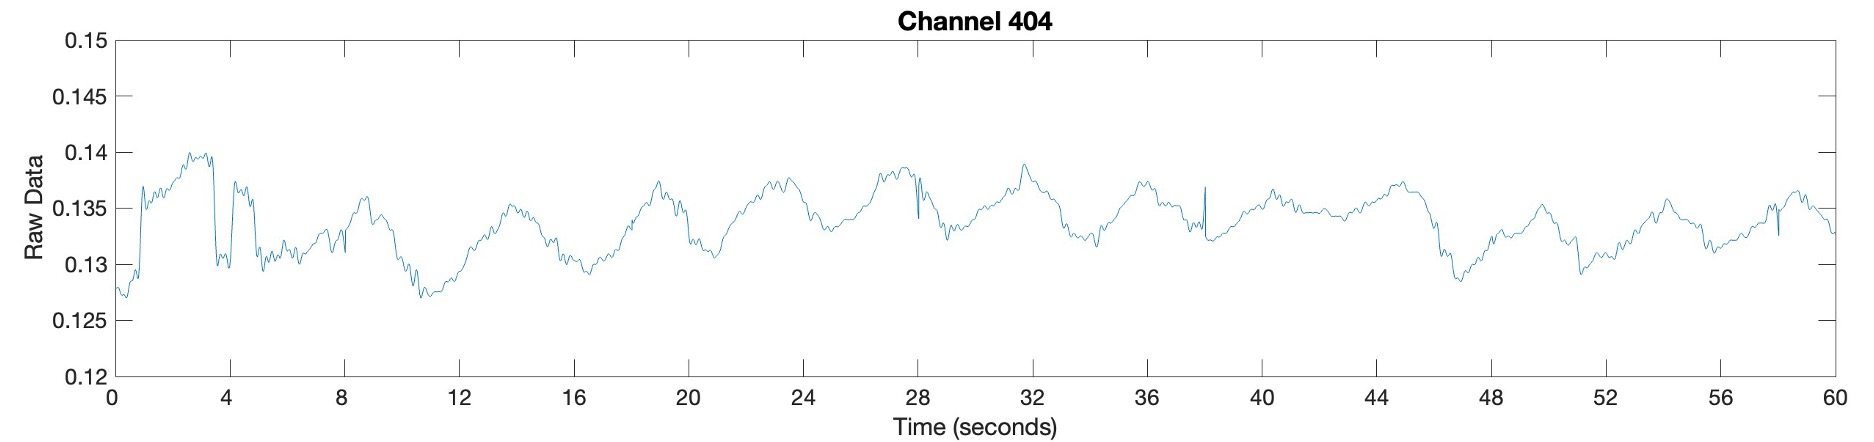
\includegraphics[width=\textwidth]{img/404.jpg}
  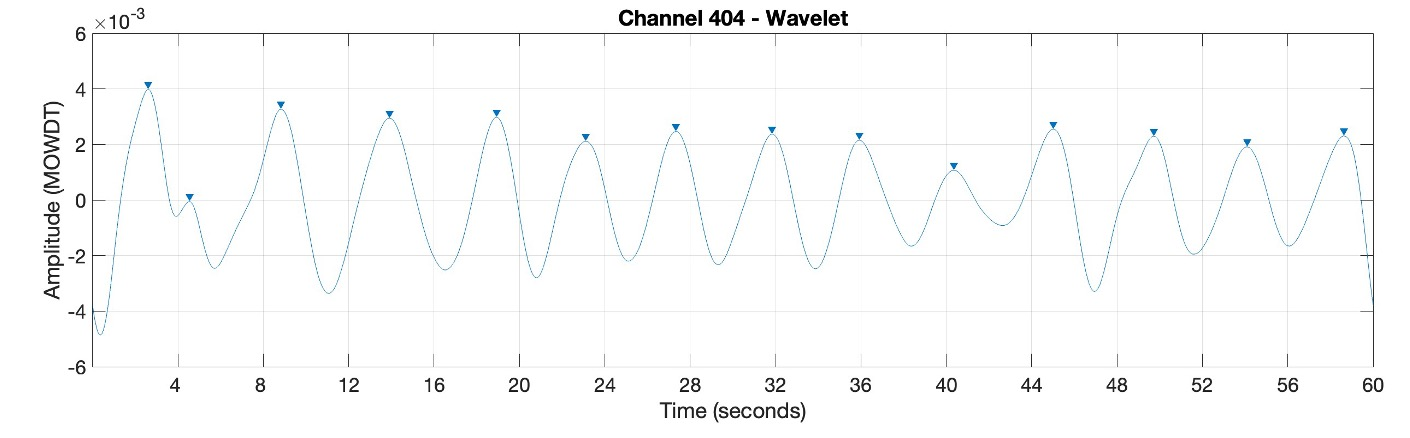
\includegraphics[width=\textwidth]{img/404_wave.jpg}
\caption{Raw data and denoised signal using MODWTMRA of the channel with the highest percentage of confidence (92\%) - Normal bed and supine position}
  \label{fig:rec}
\end{figure}



%%%%%% CONSIDERAZIONI FINALI %%%%%%
\section{Final Remarks on the Results}

This chapter presented the results of the pipeline. Since it has several parameters that can be chosen and they influence the outcome, they are commented on.

%\subsection{Evaluation of the approaches}
The pipeline allows choosing which approach to use to denoise the signal, in order to be able to give it as input to a peak finder. The different approaches are Multiresolution Overlap Discrete Wavelet Transform (described in Chapter \ref{Wavelet}) and Savitzky–Golay filter (described in Chapter \ref{sg}).
Both approaches are used in the context of the estimation of respiratory rate \cite{Sadek2017NonintrusiveStudy, Chen2008UnconstrainedSleep}, for this reason, it has been very important to have the possibility to compare them to understand which one could perform better in the context of this thesis.

The result presented in the previous section highlighted how the Savitzky–Golay filter has a lower error in respect of the wavelet approach. In fact, focusing on the MAPE it is 10\% lower in most of the positions and in both settings. The average error is 1 breath in respect of MODWTMRA which arrive up to 4 in the case of a prone position with a rocking bed.


%\subsection{Evaluation of the settings}

One of the aims of the data collection conducted during this study, described in Chapter \ref{cap:dataCollection}, has been to understand if the movement of the rocking bed could influence the signal from the mattress.
Even if the bed is designed to have an inaudible rocking mechanism, it is reasonable to expect that the movement could influence the data acquisition. The raw data visually present more noise, but the denoise approaches are able to exclude it and estimate the respiratory rate.
This can be seen in the reconstruction of the data, as shown in figure [PLACEHOLDER], and also in the result of the metrics that have a slight increase of the error but not higher as expected.
From the respiratory rate point of view, the influence on the error is mostly given by the chosen approach rather than the bed set. 

The position of the participant on the bed also seems to be decisive, in the prone position the error increases particularly and in the supine has the minimum error. It may depend on the movement of the chest that in the prone position changes.\\


\begin{comment}

%\begin{table}[h]
    \centering
    \begin{tabular}{|c|c|c|c|}
    \hline 
    Binary SGf & binary Waveleft & weighed  SGf & weighed Waveleft  \\%resp rate & toolbox \\ 
    \hline 
    12.8529 & 14.8438 & 12.8333 & 14.7353 \\ %& 13.485 & 14 \\ %
    12.0909 & 14 & 12.0909 & 14  \\ % & 13.1443 & 13 \\ 
    11.9167 & 15.125 & 11.9167 & 15.125 \\ %& 12.5154 & 13 \\ 
    13.3333 & 13.8333 & 13.4 & 13.8333 \\ %& 13.117 & 13 \\ 
    12.2857 & 14.4286 & 12.2857 & 14.4286 \\ %& 13.6077 & 14 \\ 
    12.5833 & 15.5 & 12.3077 & 15.5 \\ %& 13.8993& 15 \\ 
    11.6 & 15 & 11.6 & 15 \\ %& 12.0681 & 15 \\ 
    9 & 11 & 9 & 11 \\ %& 11.4768 & 15 \\ 
    11.1667 & 14.3333 & 10.625 & 14.3333 \\ %& 12.1549 & 14 \\ 
    14.5 & 17 & 14.5 & 17 \\ %& 12.8028 & 13 \\ 
    14.3333 & 15 & 14.3333 & 15 \\ %& 12.3275 & 14 \\ 
    11.625 & 14.1667 & 11.625 & 14.1667 \\ %& 10.9785 & 11 \\ 
    13.125 & 15.125 & 13.125 & 15.125 \\ %& 11.8441 & 11 \\ 
    13.1111 & 14.7778 & 13.1111 & 14.7778 \\ %& 12.6438 & 10 \\ 
    13.3077 & 15 & 13.3077 & 15 \\ %& 11.5351 & 11 \\ 
    13.6667 & 14 & 13.6667 & 14 \\ %& 11.99 & 10 \\ 
    11.5 & 14.2222 & 11.5 & 14.2222 \\ %& 11.9868 & 10 \\ 
    11.4545 & 14.1667 & 11.2308 & 13.8571 \\ %& 11.7824 & 10 \\ 
    \hline 
    \end{tabular}
    \caption{Breath per minute for each approach, results from Noxtural
    - A back position on a normal mattress}
\end{table}


\begin{table}[h]
\centering
\begin{tabular}{|c|c|c|c|c|}
\hline 
& Binary SGf & binary Waveleft & weighed  SGf & weighed Waveleft \\ 
\hline 
RMSE resp & 
    1.2517  &  2.4000  &  1.3043  &  2.3806 \\ 
RMSE tool &      2.4481  &  2.9583   & 2.4960  &  2.9332 \\ 
MAE resp & 1.0796 &   2.1731 &     1.1422 &  2.1499 \\ 
MAE tool &     2.0256 & 2.4179 & 2.0633 &  2.3947 \\ 
MAPE resp & 8.7793 & 17.8104 & 9.2789 & 17.6198 \\ 
MAPE tool & 16.3648 & 21.3416 & 16.5938 & 21.1266 \\ 
\hline 
\end{tabular}

\caption{Metrics to evaluate the participant in back position with still mattress}
\end{table}




\subsubsection{Back position with moving mattress}
\begin{table}[h]
\centering
\begin{tabular}{|c|c|c|c|}
\hline 
Binary SGf & binary Waveleft & weighed  SGf & weighed Waveleft  \\% & resp rate & toolbox \\ 
\hline 
14.1667 & 15.5 & 14.1667 & 15.5 \\% & 10.7609 & 8 \\ 
14.0667 & 16.1333 & 14.0667 & 16.1333 \\% & 11.3077 & 6 \\ 
13.5 & 15.3333 & 13.5 & 15.3333 \\% & 13.1449 & 8 \\ 
13.75 & 14.9474 & 13.75 & 14.9474 \\% & 11.3366 & 8 \\ 
12.9474 & 15.1 & 12.9474 & 15.1 \\% & 12.7314 & 6 \\ 
12.4615 & 15.6364 & 12.4615 & 15.6364 \\% & 11.8892 & 9 \\ 
12.6875 & 14.6923 & 12.6875 & 14.6923 \\% & 11.42 & 9 \\ 
13.5 & 15.2222 & 13.6364 & 15.2222 \\% & 13.0092 & 10 \\ 
14.6154 & 15.1667 & 14.6154 & 15.1667 \\% & 13.2539 & 12 \\ 
13.1429 & 14.6667 & 13.1429 & 14.6667 \\% & 11.6391 & 11 \\ 
14.375 & 15 & 14.375 & 15 \\% & 12.2165 & 11 \\ 
15.4286 & 14.75 & 15.4286 & 14.75 \\% & 11.9216 & 12 \\ 
14.6667 & 15 & 14.6667 & 15 \\% & 11.3091 & 13 \\ 
14.8182 & 14.625 & 14.8182 & 14.625 \\% & 13.8905 & 12 \\ 
14.5385 & 15.6154 & 14.5385 & 15.6154 \\% & 11.3344 & 13 \\ 
13.9091 & 15 & 13.9167 & 14.8182 \\% & 11.4474 & 11 \\ 
13.8824 & 15.1765 & 13.8824 & 15.1765 \\% & 11.6675 & 11 \\ 
13.8667 & 14.6154 & 13.8667 & 14.6154 \\% & 13.4799 & 12 \\ 
\hline 
\end{tabular}


\caption{Breath per minutes for each approach, result from Noxtural and toolbox  - Back position moving mattress}

\end{table}


\begin{table}[h]

    \centering

\begin{tabular}{|c|c|c|c|c|}
\hline 
& Binary SGf & binary Waveleft & weighed  SGf & weighed Waveleft \\ 
 
\hline 
RMSE resp &  2.1340  &  3.2155  &  2.1365  &  3.2047 \\ 
RMSE tool &     4.2192  &  5.5405  &  4.2259   & 5.5334 \\  
MAE resp & 1.8091 &   3.0234 &     1.8171 &  3.0133 \\ 
MAE tool &     3.7957 & 5.0100 & 3.8037 &  4.9999 \\  
MAPE resp & 15.5385 & 25.7324 & 15.6004 & 25.6442 \\ 
MAPE tool & 44.4027 & 58.5849 & 44.4823 & 58.4931 \\ 

\hline 
\end{tabular}

\caption{Metrics to evaluate the participant in back position with moving mattress}
\end{table}


\subsubsection{Left position with still mattress}
\begin{table}\begin{tabular}{|llllll|}
\hline 
Binary SGf & binary Waveleft & weighed  SGf & weighed Waveleft & resp rate & toolbox \\ 
\hline 
13.375 & 14.6364 & 13.375 & 14.6364 & 11.2045 & 10 \\ 
13.6667 & 15 & 13.6667 & 15 & 12.7397 & 11 \\ 
14 & 16 & 13.5 & 15.25 & 13.0613 & 12 \\ 
14.3571 & 14.2 & 14.3571 & 14.2 & 12.2669 & 12 \\ 
14 & 19 & 14 & 19 & 12.1628 & 13 \\ 
12.8 & 15 & 12.6667 & 14.5 & 13.6039 & 13 \\ 
11.8 & 14.2222 & 11.8 & 14.2222 & 13.1398 & 13 \\ 
14 & 15.6667 & 14 & 15.6667 & 11.5445 & 14 \\ 
13.8333 & 14.7 & 13.8333 & 14.7 & 10.77 & 11 \\ 
13.8889 & 15.8571 & 13.8889 & 15.8571 & 14.2216 & 12 \\ 
13.0833 & 15.5556 & 13.0833 & 15.5556 & 13.1656 & 12 \\ 
14.1111 & 16.5714 & 13.7 & 16.5714 & 12.9764 & 12 \\ 
14.2 & 15 & 14.2 & 15 & 10.9055 & 13 \\ 
13.25 & 15.125 & 13.25 & 15.125 & 13.2294 & 11 \\ 
12.7692 & 15.7143 & 12.2857 & 15.5 & 12.8524 & 11 \\ 
13.9167 & 15.2 & 13.6154 & 15.2 & 11.3824 & 13 \\ 
13 & 14.6 & 13 & 14.6 & 13.5579 & 11 \\ 
13 & 15.8889 & 13 & 15.8889 & 11.6069 & 12 \\ 
\hline 
\end{tabular}
\caption{Breath per minutes for each approach, result from Noxtural and toolbox
- Left position still mattress}
\end{table}

\begin{table}
\begin{tabular}{|lllll|}
\hline 
& Binary SGf & binary Waveleft & weighed  SGf & weighed Waveleft \\ 

\hline 
RMSE resp &
      1.7158  &  3.2950  &  1.6774  &  3.2425 \\
RMSE  tool &    1.8743  &  3.6582   & 1.7959   & 3.5879 \\
MAE resp & 1.3922 &   2.4545 &     1.3591 &  2.8934 \\ 
MAE tool &     1.6584 & 2.9748 & 1.5716 &  3.3596 \\
MAPE resp & 11.8278 & 24.62 & 11.5556 & 24.0041 \\ 
MAPE tool & 14.4565 & 29.3635 & 13.7188 & 28.6943 \\ 
\hline 
\end{tabular}

\caption{Metrics to evaluate the participant in left position with still mattress}
\end{table}


%\section{Left position with moving mattress}
\begin{table}
\begin{tabular}{|llllll|}
\hline 
Binary SGf & binary Waveleft & weighed  SGf & weighed Waveleft & resp rate & toolbox \\ 
\hline 
13.6875 & 15.0625 & 13.6875 & 15.0625 & 13.6613 & 11 \\ 
14.5294 & 15.5556 & 14.5294 & 15.5556 & 11.4545 & 8 \\ 
14.5 & 15.8824 & 14.5 & 15.8824 & 12.3288 & 6 \\ 
13.9444 & 16.1176 & 13.9444 & 16.1176 & 10.8865 & 7 \\ 
14.0455 & 15.2083 & 14.0455 & 15.2083 & 11.4082 & 9 \\ 
13.44 & 15.3214 & 13.4231 & 15.3103 & 12.2589 & 6 \\ 
13.9091 & 15.4583 & 13.9091 & 15.4583 & 13.7093 & 8 \\ 
14 & 15.4375 & 14 & 15.4375 & 12.7019 & 10 \\ 
14.4 & 15.2353 & 14.4 & 15.2353 & 13.3305 & 12 \\ 
14.5769 & 15.5556 & 14.5769 & 15.5556 & 13.7078 & 13 \\ 
14.7 & 15.2143 & 14.7 & 15.2143 & 13.5674 & 14 \\ 
14.8421 & 15.2 & 14.8421 & 15.1538 & 11.8694 & 15 \\ 
14.85 & 15.5556 & 14.85 & 15.5556 & 13.4086 & 15 \\ 
15.5 & 14.75 & 15.5 & 14.75 & 13.9781 & 15 \\ 
13.6667 & 14.5 & 13.6667 & 14.5 & 12.4749 & 13 \\ 
13.8571 & 15.25 & 13.8571 & 15.25 & 12.4049 & 13 \\ 
13.375 & 14.625 & 13.7 & 14.7273 & 13.4108 & 12 \\ 
13.75 & 14.2857 & 14.1667 & 14.3333 & 13.4716 & 14 \\ 
\hline 
\end{tabular}
\caption{Breath per minutes for each approach, result from Noxtural and toolbox
- Left position moving mattress}
\end{table}

\begin{table}

\begin{tabular}{|lllll|}
\hline 
& Binary SGf & binary Waveleft & weighed  SGf & weighed Waveleft \\ 

\hline 
RMSE resp &
      1.7259  &  2.7236  &  1.7331   & 2.7232 \\
RMSE  tool &   4.1782  &  5.2608  &  4.1829   & 5.2627 \\
MAE resp & 1.4229 &   2.4545 &     1.4592 &  2.4597 \\ 
MAE tool &     3.0939 & 4.0953 & 3.1063 &  4.1004 \\
MAPE resp & 11.6751 & 19.9605 & 11.9443 & 19.9959 \\ 
MAPE tool & 39.3516 & 50.7242 & 39.4533 & 50.7631 \\ 
\hline 
\end{tabular}

\caption{Metrics to evaluate the participant in left position with moving mattress}
\end{table}



%\section{Belly position with still mattress}
\begin{table}
\begin{tabular}{|llllll|}
\hline 
Binary SGf & binary Waveleft & weighed  SGf & weighed Waveleft & resp rate & toolbox \\ 
\hline 
15.3 & 15.7 & 15.3 & 15.7 & 11.5949 & 14 \\ 
14.8125 & 15.7333 & 14.8125 & 15.7333 & 11.1628 & 16 \\ 
14.2 & 16.1 & 14.2 & 16.1 & 11.0005 & 16 \\ 
14.8889 & 15.6667 & 14.8889 & 15.6667 & 10.4762 & 15 \\ 
13.5 & 15.25 & 13.5 & 15.25 & 10.4723 & 15 \\ 
13.8571 & 14.5714 & 13.8571 & 14.5714 & 9.5345 & 14 \\ 
13.8571 & 15.5714 & 13.8571 & 15.5714 & 9.5467 & 13 \\ 
14.3 & 15.875 & 14.3 & 15.875 & 13.5758 & 14 \\ 
15 & 14 & 15 & 14 & 11.1779 & 14 \\ 
13.9 & 14.375 & 13.9 & 14.375 & 9.5345 & 14 \\ 
13.8667 & 14.4667 & 13.8667 & 14.4667 & 9.5841 & 15 \\ 
13.8235 & 14.5 & 13.8235 & 14.5 & 11.8196 & 14 \\ 
14.0714 & 14.2143 & 14.0714 & 14.2143 & 11.8153 & 10 \\ 
13 & 13.9474 & 13 & 13.9474 & 9.5223 & 8 \\ 
14.4828 & 15.037 & 14.4828 & 15.037 & 10.8508 & 8 \\ 
14.3793 & 14.931 & 14.3793 & 14.931 & 10.8876 & 7 \\ 
13.7 & 15.25 & 13.7 & 15.25 & 10.9705 & 7 \\ 
14.1818 & 15.3333 & 14.1818 & 15.3333 & 11.237 & 6 \\ 
\hline 
\end{tabular}

\caption{Breath per minutes for each approach, result from Noxtural and toolbox
- Belly position still mattress}
\end{table}


\begin{table}
\begin{tabular}{|lllll|}
\hline 
& Binary SGf & binary Waveleft & weighed  SGf & weighed Waveleft \\ 

\hline 
RMSE resp &
     3.4835  &  4.3281 &   3.4835  &  4.3281 \\
RMSE  tool & 3.8127   & 4.3162   & 3.8127  &  4.3162 \\
MAE resp & 3.3532 &   4.2088 &     3.3532 &  4.2088 \\ 
MAE tool &     2.6347 & 2.8957 & 2.6347 &  2.8957 \\
MAPE resp & 31.914 & 39.9076 & 31.914 & 39.9076 \\ 
MAPE tool & 32.6041 & 36.5982 & 32.6041 & 36.5982 \\ 
\hline 
\end{tabular}

\caption{Metrics to evaluate the participant in belly position with moving mattress}
\end{table}


%\section{Belly position with moving mattress}
\begin{table}
\begin{tabular}{|llllll|}
\hline 
Binary SGf & binary Waveleft & weighed  SGf & weighed Waveleft & resp rate & toolbox \\ 
\hline 
14.6667 & 16 & 14.6667 & 16 & 12.6296 & 9 \\ 
14.0455 & 15.3684 & 14.0455 & 15.3684 & 14.168 & 12 \\ 
14.3478 & 15.6818 & 14.3478 & 15.6818 & 13.2588 & 13 \\ 
14.381 & 15.5 & 14.3636 & 15.4286 & 13.8107 & 13 \\ 
13.7143 & 15.8333 & 13.7143 & 15.8333 & 13.485 & 13 \\ 
14 & 16 & 14 & 16 & 12.6052 & 14 \\ 
16.1 & 16 & 16.1 & 16 & 11.0417 & 17 \\ 
15.7647 & 15.7059 & 15.7647 & 15.7059 & 12.9088 & 17 \\ 
14.7333 & 15.5333 & 14.7333 & 15.5333 & 13.0502 & 16 \\ 
14.6 & 16.3333 & 14.6 & 16.3333 & 11.1723 & 17 \\ 
14.3846 & 14.5625 & 14.3846 & 14.5625 & 14.6869 & 16 \\ 
13.8889 & 15.5294 & 13.8889 & 15.5294 & 11.3484 & 13 \\ 
13.7273 & 14.7273 & 13.7273 & 14.7273 & 13.0399 & 11 \\ 
13.8235 & 14.7778 & 13.8235 & 14.7778 & 9.5487 & 10 \\ 
13.6111 & 15.4444 & 13.6111 & 15.4444 & 11.7918 & 11 \\ 
13.2667 & 14.9286 & 13.2667 & 14.9286 & 12.8182 & 8 \\ 
12.9375 & 15.8333 & 12.9375 & 15.8333 & 9.5345 & 8 \\ 
13.3 & 14.619 & 13.3 & 14.619 & 9.5416 & 13 \\ 
\hline 
\end{tabular}\caption{Breath per minutes for each approach, result from Noxtural and toolbox
- Belly position moving mattress}
\end{table}

\begin{table}
\begin{tabular}{|lllll|}
\hline 
& Binary SGf & binary Waveleft & weighed  SGf & weighed Waveleft \\ 
 
\hline 
RMSE resp &
    2.4778  &  3.6110  &  2.4775  &  3.6092 \\
RMSE  tool &  2.7357  &  3.8447  &  2.7352  &  3.8422 \\
MAE resp & 1.9835 &   3.2326 &     1.9825 &  3.2286 \\ 
MAE tool &     2.1737 & 3.2326 & 2.1728 &  3.1687 \\ 
MAPE resp & 17.8949 & 28.5509 & 17.8879 & 28.5221 \\ 
MAPE tool & 20.8138 & 30.5337 & 20.8064 & 30.5032 \\ 
\hline 
\end{tabular}

\caption{Metrics to evaluate the participant in belly position with moving mattress}
\end{table}



%\section{Right position with still mattress}
\begin{table}\begin{tabular}{|llllll|}
\hline 
Binary SGf & binary Waveleft & weighed  SGf & weighed Waveleft & resp rate & toolbox \\ 

\hline 
14.5714 & 16.1667 & 14.5714 & 16.1667 & 12.4771 & 17 \\ 
14 & 17.75 & 14 & 17.75 & 13.0835 & 17 \\ 
16.5 & 16.5 & 16.5 & 16.5 & 14.3858 & 17 \\ 
14.7778 & 15.25 & 14.7778 & 15.25 & 12.7261 & 17 \\ 
14.5 & 15.8333 & 14.5 & 15.8333 & 13.4867 & 17 \\ 
13.9333 & 15 & 13.9333 & 15 & 12.9816 & 16 \\ 
15 & 15.2353 & 15 & 15.2353 & 14.0566 & 15 \\ 
13.7692 & 15.1667 & 13.7692 & 15.1667 & 12.038 & 16 \\ 
14 & 15.5 & 14 & 15.5 & 11.4923 & 12 \\ 
14.6 & 13 & 14.6 & 13 & 11.9625 & 10 \\ 
15 & 13.3333 & 14.3333 & 13.5 & 11.0151 & 9 \\ 
16.5 & 15.5 & 16.5 & 15.5 & 11.9016 & 10 \\ 
14.5 & 14.3333 & 14.5 & 14.3333 & 11.4255 & 10 \\ 
12.2857 & 13.8333 & 12.2857 & 13.8333 & 12.5227 & 7 \\ 
12.8333 & 15.2 & 12.8333 & 15.2 & 11.5945 & 10 \\ 
12.3333 & 14.0909 & 12.3333 & 14.0909 & 13.4141 & 8 \\ 
12.3636 & 14.5 & 12.4783 & 14.4286 & 13.5282 & 11 \\ 
13.4286 & 15.2308 & 12.875 & 15.2308 & 12.9839 & 11 \\ 
\hline 
\end{tabular}
\caption{Breath per minutes for each approach, result from Noxtural and toolbox
- Right position still mattress}
\end{table}
\begin{table}\begin{tabular}{|lllll|}
\hline 
& Binary SGf & binary Waveleft & weighed  SGf & weighed Waveleft \\ 
\hline 
RMSE resp &
     2.1572  &  2.7087  &  2.0877  &  2.7156 \\
RMSE  tool &    3.5099  &   3.6341   & 3.4330 &   3.6416 \\
MAE resp & 1.8214 &   2.4638 &     1.7593 &  2.4691 \\ 
MAE tool &     3.0440 & 2.9772 & 2.9826 &  2.9825 \\
MAPE resp & 14.9336 & 19.9146 & 14.4066 & 19.9693 \\ 
MAPE tool & 28.9627 & 30.229 & 28.3295 & 30.2958 \\ 
\hline 
\end{tabular}

\caption{Metrics to evaluate the participant in right position with still mattress}
\end{table}


%\section{Right position with moving mattress}
\begin{table}\begin{tabular}{|llllll|}
\hline 
Binary SGf & binary Waveleft & weighed  SGf & weighed Waveleft & resp rate & toolbox \\ 
\hline 
14.2273 & 15.8095 & 14.2273 & 15.8095 & 11.7955 & 10 \\ 
13.625 & 15.2105 & 13.5294 & 15.1 & 11.9185 & 9 \\ 
13.9524 & 15.5652 & 13.9524 & 15.5652 & 11.8639 & 8 \\ 
15 & 15.8261 & 14.7826 & 15.8261 & 12.28 & 10 \\ 
14.5652 & 15.6667 & 14.375 & 15.6667 & 12.0136 & 10 \\ 
13.625 & 15.1176 & 13.625 & 15.1176 & 12.8838 & 10 \\ 
14.4118 & 15.3571 & 14.4118 & 15.3571 & 11.5695 & 12 \\ 
14.72 & 15 & 14.72 & 14.8696 & 12.8922 & 13 \\ 
14.85 & 15.1176 & 14.85 & 15.1176 & 11.587 & 14 \\ 
15 & 15.2857 & 15 & 15.2857 & 11.2449 & 14 \\ 
15.2917 & 15.3333 & 15.28 & 15.3333 & 11.7082 & 15 \\ 
15.5294 & 15.3684 & 15.5 & 15.35 & 13.9497 & 15 \\ 
14.5625 & 15.6154 & 14.5294 & 15.4286 & 11.6145 & 16 \\ 
14.8182 & 15.4286 & 14.8182 & 15.4286 & 13.9913 & 16 \\ 
14.7333 & 15.2727 & 14.7333 & 15.2727 & 11.6172 & 16 \\ 
14.8824 & 15.3 & 14.8824 & 15.3 & 13.3257 & 16 \\ 
14.75 & 15.1667 & 14.75 & 15.1667 & 13.5179 & 16 \\ 
15.0667 & 14.9231 & 15.0667 & 14.9286 & 13.5767 & 16 \\ 
\hline 
\end{tabular}
\caption{Breath per minutes for each approach, result from Noxtural and toolbox
- Right position moving mattress}
\end{table}

\begin{table}\begin{tabular}{|lllll|}
\hline 
& Binary SGf & binary Waveleft & weighed  SGf & weighed Waveleft \\ 

\hline 
RMSE resp &
     2.4083   & 3.1106  &  2.3763 &   3.0860 \\
RMSE  tool &    2.9182  &  3.6785   & 2.8737  &  3.6656 \\
MAE resp & 2.2367 &   2.9452 &     2.2046 &  2.9208 \\ 
MAE tool &     2.3325 & 2.7195 & 2.3041 &  2.7152 \\
MAPE resp & 18.5442 & 24.4008 & 18.2803 & 24.1986 \\ 
MAPE tool & 22.0502 & 26.6562 & 21.761 & 26.5883 \\ 
\hline 
\end{tabular}

\caption{Metrics to evaluate the participant in right position with moving mattress}
\end{table}

\end{comment}
\chapter{Conclusion and future discussin}
\listoftables
\listoffigures
\bibliographystyle{ieeetr}
\bibliography{biblio}




\fancyhead[LO,RE]{\slshape \leftmark}
%\fancyhead[CO,CE]{\slshape\rightmark}
\fancyhead[LE,RO]{}
%\addcontentsline{toc}{chapter}{Bibliografia}
%\bibliographystyle{unsrt}
%\bibliography{thesis}

\end{document}

